%% ============================================================
%% Agentic AI-Based 5G Network Slice Orchestrator — Major Project Report
%% KLE Technological University, Hubballi
%% ============================================================
\documentclass[12pt,a4paper]{report}

\usepackage[a4paper, top=25mm, bottom=25mm, left=35mm, right=20mm]{geometry}
\usepackage{graphicx}
\usepackage{amsmath, amssymb, mathtools}
\usepackage{booktabs}
\usepackage{longtable}
\usepackage{array}
\usepackage{multirow}
\usepackage{tabularx}
\usepackage[hidelinks]{hyperref}
\usepackage[dvipsnames,svgnames,table]{xcolor}
\usepackage{listings}
\usepackage{caption}
\usepackage{subcaption}
\usepackage{fancyhdr}
\usepackage{setspace}
\usepackage{enumitem}
\usepackage{titlesec}
\usepackage{float}
\usepackage{algorithm}
\usepackage{algpseudocode}
\usepackage{microtype}
\usepackage{parskip}
\usepackage{lmodern}
\usepackage[T1]{fontenc}
\usepackage{rotating}
\usepackage{pgfplots}
\usepackage{pgfplotstable}
\usepackage{tikz}
\usepackage{cite}
\usepackage[most]{tcolorbox}
\setlength{\headheight}{14.5pt}

\pgfplotsset{compat=1.18}
\usetikzlibrary{shapes.geometric, shapes.misc, arrows.meta, positioning,
                decorations.pathreplacing, calc, backgrounds, fit, matrix}

%% Page style
\pagestyle{fancy}
\fancyhf{}
\fancyhead[R]{\small Agentic AI-Based 5G Network Slice Orchestrator}
\fancyfoot[C]{\thepage}
\renewcommand{\headrulewidth}{0.4pt}

%% Chapter title format
\titleformat{\chapter}[block]
  {\normalfont\Large\bfseries\centering}{Chapter \thechapter}{1em}{}
\titlespacing*{\chapter}{0pt}{30pt}{20pt}

%% Listings
\lstset{
  basicstyle=\ttfamily\small,
  breaklines=true, breakatwhitespace=true,
  frame=single,
  backgroundcolor=\color{gray!8},
  keywordstyle=\color{blue}\bfseries,
  commentstyle=\color{green!60!black},
  stringstyle=\color{red!60!yellow},
  numbers=left, numberstyle=\tiny\color{gray},
  numbersep=5pt, xleftmargin=12pt,
  captionpos=b
}

%% Algorithm style tweaks
\algrenewcommand\algorithmicindent{1.2em}
\algrenewcommand{\algorithmicrequire}{\textbf{Input:}}
\algrenewcommand{\algorithmicensure}{\textbf{Output:}}

%% Colours — project palette
\definecolor{agentblue}{RGB}{30,100,190}
\definecolor{slicegreen}{RGB}{40,160,80}
\definecolor{urllcred}{RGB}{200,50,50}
\definecolor{embbblue}{RGB}{50,100,200}
\definecolor{mmtcgray}{RGB}{100,120,100}
% Extended palette matching reports/architectures.pdf
\definecolor{cran}{HTML}{4B5563}
\definecolor{c5g}{HTML}{1E3A5F}
\definecolor{cembb}{HTML}{1D4ED8}
\definecolor{curllc}{HTML}{DC2626}
\definecolor{cmmtc}{HTML}{15803D}
\definecolor{cqos}{HTML}{D97706}
\definecolor{cprom}{HTML}{EA580C}
\definecolor{cgraf}{HTML}{0D9488}
\definecolor{corch}{HTML}{7C3AED}
\definecolor{ccontrib}{HTML}{1E40AF}

%% Contribution box style
\tcbuselibrary{skins,breakable}
\newtcolorbox{contribbox}[1]{
  colback=ccontrib!5, colframe=ccontrib!60,
  fonttitle=\bfseries\small, title=#1,
  breakable, left=6pt, right=6pt, top=4pt, bottom=4pt,
  arc=4pt
}

\begin{document}

%% ---- Cover Page
\begin{titlepage}
\centering
{\large\bfseries SCHOOL OF COMPUTER SCIENCE AND ENGINEERING}\\[0.3cm]
{\large KLE Technological University, Hubballi -- 580031}\\[1cm]
\rule{\linewidth}{0.5pt}\\[0.4cm]
{\Large\bfseries Major Project Report}\\[0.3cm]
{\large On}\\[0.5cm]
{\LARGE\bfseries Agentic AI-Based 5G Network Slice Orchestrator:\\[0.2cm]
Autonomous QoS Management using Large Language Models\\[0.2cm]
and Multi-Agent Reasoning}\\[0.5cm]
\rule{\linewidth}{0.5pt}\\[0.5cm]
{\normalsize submitted in partial fulfillment of the requirements for the award of the degree of}\\[0.4cm]
{\large\bfseries Bachelor of Engineering}\\
{\normalsize in}\\
{\large\bfseries COMPUTER SCIENCE AND ENGINEERING}\\[1.2cm]
{\normalsize\bfseries Submitted By}\\[0.4cm]
\begin{tabular}{ll}
Simran R Kalkeri       & 01FE23BCI087 \\[4pt]
Amaanali D Doddamani   & 01FE23BCI091 \\[4pt]
Sparsh Sunil Naik      & 01FE23BCI085 \\[4pt]
Rishi P Kulkarni       & 01FE23BCI088 \\
\end{tabular}\\[1.2cm]
{\normalsize Under the guidance of}\\[0.3cm]
{\large\bfseries Dr.\ Narayan D G}\\
{\normalsize Professor, School of Computer Science and Engineering}\\[0.5cm]
{\normalsize KLE Technological University, Hubballi}\\[1cm]
{\large 2025--2026}
\end{titlepage}

%% ---- Certificate
\newpage\thispagestyle{empty}
\begin{center}{\Large\bfseries CERTIFICATE}\end{center}
\vspace{1cm}
\noindent
This is to certify that the project entitled \textbf{``Agentic AI-Based 5G Network Slice Orchestrator: Autonomous QoS Management using Large Language Models and Multi-Agent Reasoning''} is a bona fide work carried out by the student team (Simran R Kalkeri -- 01FE23BCI087, Amaanali D Doddamani -- 01FE23BCI091, Sparsh Sunil Naik -- 01FE23BCI085, Rishi P Kulkarni -- 01FE23BCI088), in partial fulfillment of the requirements for the 6th semester B.E.\ course during the academic year 2025--2026. The project report has been approved as it satisfies the academic requirements prescribed for the said course.
\vspace{2cm}\\
\begin{tabular}{p{6cm}p{6cm}}
Dr.\ Narayan D G & Dr.\ Meena S.\ M. \\
\textit{Guide} & \textit{Head of the Department}
\end{tabular}
\vspace{2cm}
\begin{center}{\bfseries External Viva-Voce}\end{center}
\begin{tabular}{p{9cm}p{5cm}}
Name of the Examiner & Signature with Date \\[0.8cm]
1.\ \dotfill & \dotfill \\[0.8cm]
2.\ \dotfill & \dotfill \\
\end{tabular}

%% ---- Acknowledgement
\newpage\thispagestyle{empty}
\chapter*{Acknowledgement}
\addcontentsline{toc}{chapter}{Acknowledgement}
We express our sincere gratitude to our faculty and management for their professional guidance and support throughout the course of this project. We thank Dr.\ Ashok Shettar, Vice-Chancellor, Dr.\ B.S.\ Anami, Registrar, and Dr.\ P.G.\ Tewari, Dean Academics, KLE Technological University, Hubballi, for their vision and institutional support.

We acknowledge Dr.\ Meena S.\ M., Professor and Head, SoCSE, for providing direction and facilitating an environment conducive to academic growth and engineering innovation.

We sincerely thank our guide, Dr.\ Narayan D G, Professor, SoCSE, for his unwavering guidance, invaluable suggestions, and constant encouragement throughout the design, implementation, and evaluation phases of this project.

We extend our gratitude to Mr.\ Naveen Kumar for helping us navigate the complex landscape of cloud-native 5G infrastructure and Kubernetes-based deployments. We also thank project coordinators Mr.\ Uday N.\ Kulkarni and Mr.\ Guruprasad Konnuramath for their administrative support.

\vspace{2cm}
\begin{flushright}
Simran R Kalkeri -- 01FE23BCI087 \\
Amaanali D Doddamani -- 01FE23BCI091 \\
Sparsh Sunil Naik -- 01FE23BCI085 \\
Rishi P Kulkarni -- 01FE23BCI088
\end{flushright}

%% ---- Abstract
\newpage
\chapter*{ABSTRACT}
\addcontentsline{toc}{chapter}{ABSTRACT}
Network slicing is a foundational capability of 5G networks, enabling simultaneous support of enhanced Mobile Broadband (eMBB), Ultra-Reliable Low-Latency Communication (URLLC), and massive Machine-Type Communication (mMTC) on shared physical infrastructure. While prior work has demonstrated static and rule-based adaptive slicing, these approaches cannot reason about root causes of QoS degradation or adapt decisions based on accumulated operational experience.

This project presents the design, implementation, and evaluation of an \textbf{Agentic AI-Based 5G Network Slice Orchestrator}: a fully autonomous closed-loop control system in which a Large Language Model (LLM) backed agent performs slice-level QoS orchestration. The system is built on an Open5GS 5G Standalone core, UERANSIM-based RAN emulation, and a Kubernetes-managed user-plane deployment with per-slice traffic shaping via Linux \texttt{tc}. A LangGraph multi-agent architecture---comprising a Monitoring Agent, Planning Agent, Execution Agent, and Agent Memory---implements a structured observe$\rightarrow$think$\rightarrow$validate$\rightarrow$act$\rightarrow$reflect control loop.

Six research contributions are made: (1) an Autonomous QoS Orchestration Framework, (2) a LangGraph Multi-Agent Architecture, (3) a Chain-of-Thought Network Reasoning schema requiring explicit \texttt{root\_cause\_assessment} and \texttt{lever\_validity} fields, (4) a Wrong-Lever Avoidance Mechanism using a novel relative load metric \texttt{embb\_load\_fraction}, (5) a Memory-Assisted Decision subsystem providing historical context, and (6) a rigorous Comparative Evaluation against a rule-based baseline.

Experimental results demonstrate: 96.3\% URLLC SLA compliance (vs. 87.1\%), 4.2\,s mean recovery time (vs. 8.4\,s), 72\% reduction in eMBB throughput loss, and full Chain-of-Thought decision traces for post-hoc audit.

\vspace{0.5cm}
\noindent\textbf{Keywords:} 5G Network Slicing, Autonomous Orchestration, Large Language Model, Chain-of-Thought Reasoning, Quality of Service, LangGraph, Multi-Agent System, Open5GS, Kubernetes, URLLC, eMBB, mMTC

%% ---- TOC / LOT / LOF
\newpage\tableofcontents
\newpage\listoftables
\newpage\listoffigures

\pagenumbering{arabic}\setcounter{page}{1}

%% ---- Include chapters
%% ch1_introduction.tex

\chapter{INTRODUCTION}

Fifth Generation (5G) mobile networks introduce network slicing as a defining architectural capability, enabling multiple logical network instances---each with distinct performance characteristics---to coexist on shared physical infrastructure. Network slicing permits concurrent support of enhanced Mobile Broadband (eMBB), Ultra-Reliable Low-Latency Communication (URLLC), and massive Machine-Type Communication (mMTC) services, each with fundamentally different QoS requirements. eMBB demands high throughput and tolerates moderate latency; URLLC requires end-to-end latencies below 20\,ms with very high reliability; and mMTC targets energy-efficient transmission for large-scale IoT device populations.

Realising these guarantees in practice is challenging. At the user plane, traffic from different slices may contend for shared buffering and forwarding resources during congestion. Static resource allocations fail to track dynamic traffic demands, while reactive threshold-based controllers lack the ability to reason about the root cause of degradation or to anticipate violations before they occur.

Autonomous orchestration, enabled by Large Language Models (LLMs) and multi-agent frameworks, offers a qualitatively different control paradigm. Rather than pattern-matching against hardcoded thresholds, an LLM-based planning agent performs causal reasoning: identifying which network entity is responsible for congestion, validating whether the proposed control action addresses that cause, and consulting prior operational history stored in an agent memory to refine its decisions. This project implements, deploys, and evaluates such a system in a cloud-native 5G testbed.

\section{Motivation}

The evolution from rule-based to autonomous orchestration is driven by three limitations observed in practical 5G slice management systems.

\textbf{First}, rule-based controllers are structurally blind to causation. A threshold-based system that detects elevated URLLC RTT will throttle eMBB bandwidth regardless of whether eMBB traffic is actually active. When eMBB load is low, this action is unnecessary and harmful. An agent capable of reasoning about relative load---quantified by the \texttt{embb\_load\_fraction} metric introduced in this work---can correctly distinguish idle from bursting eMBB and decline to act when throttling is ineffective.

\textbf{Second}, reactive control cannot prevent violations; it can only respond to them. A URLLC SLA breach lasting even 200\,ms may disrupt a latency-critical industrial automation session. Pre-emptive action, triggered by trend analysis and predictive causal reasoning, is only possible when the controller possesses a causal model of the network state rather than a simple threshold table.

\textbf{Third}, accumulated operational experience is wasted in memoryless systems. An agent that stores the outcome of prior actions---including whether throttling eMBB at a given load level subsequently resolved the RTT violation---can converge to more accurate control policies over time without requiring offline training.

\section{Literature Survey}

\textbf{Bandara et al.} propose an AI-native framework for 6G network slice orchestration, monitoring, and trading using multiple autonomous AI agents and Large Language Models (LLMs)~\cite{bandara2026}. The architecture consists of layered components that perform intent interpretation, slice deployment, SLA monitoring, policy enforcement, and resource allocation. The framework integrates the Model Context Protocol (MCP) to translate natural language requests into secure orchestration actions and was evaluated on an Open5GS, Ericsson RAN, and Kubernetes testbed.

\textbf{Grings et al.} propose a full dynamic orchestration framework for 5G core network slicing over a cloud-native Kubernetes platform~\cite{grings2022}. Unlike existing approaches that only support partial orchestration through resource scaling, the proposed solution introduces a Kubernetes-integrated controller capable of dynamically reconfiguring 5G core functions, including NSSF, AMF, SMF, and UPF, during runtime without terminating active network slices, reducing reconfiguration requests by approximately 47.5\%.

\textbf{Novanana et al.} propose a Kubernetes-based MANO framework for provisioning coexisting eMBB and URLLC services through 5G network slicing using open-source technologies~\cite{novanana2024}. The authors integrate free5GC, UERANSIM, OpenStack, and kube5gnfvo to evaluate separate UPF vs. dedicated SMF/UPF configurations, showing that dedicated SMF/UPF pairs deliver better performance, achieving a stable throughput of 20.2--22.1\,Gbps and improved congestion control.

\textbf{Reddy} proposes a Deep Reinforcement Learning (DRL)-based Kubernetes autoscaling framework for managing high-throughput 5G network functions and slices using a Deep Q-Learning (DQN) agent~\cite{reddy2025}. The system dynamically scales Kubernetes pods based on real-time network conditions. Experimental results show 71.7\% faster slice deployment, 35\% higher resource utilization, 22\% lower latency, 40\% faster processing times, and up to 96.7\% spectrum efficiency compared to conventional methods.

\textbf{Dandoush et al.} propose an LLM-powered network slicing management and orchestration framework that integrates Large Language Models (LLMs) and multi-agent systems with ETSI MANO and 3GPP slicing architectures~\cite{dandoush2024}. The conceptual framework enables LLM agents to translate natural language intent into technical slice requirements, automate slice design and deployment, coordinate multi-domain resources, and manage performance without needing hardcoded rules.

\textbf{Sulaiman et al.} propose MicroOpt, a model-driven framework for dynamic resource optimization in 5G network slicing that uses a differentiable deep neural network (DNN) and gradient-based optimization to allocate resources~\cite{sulaiman2024}. The system predicts traffic, models QoS, and uses a primal-dual optimization algorithm to dynamically scale CPU and bandwidth. Deployed on an open-source testbed with srsRAN, Open5GS, Kubernetes, and Prometheus, it achieved up to 21.9\% lower resource consumption.

\textbf{Saha et al.} propose MonArch, a scalable monitoring architecture for cloud-native 5G deployments that integrates Prometheus, Elasticsearch, Apache Kafka, Logstash, and Kubernetes to collect, correlate, and analyze monitoring data across slices~\cite{saha2022}. Tested on a Kubernetes-based 5G testbed using Free5GC and UERANSIM, MonArch demonstrated minimal data-ingestion overhead and efficient scaling using a 5-second monitoring interval.

\textbf{Tran et al.} propose PCLANSA, a machine-learning-based closed-loop service assurance framework for 5G and B5G network slicing~\cite{tran2025}. The framework uses LSTM-based traffic prediction to forecast future demand and automatically perform VNF scaling and link-capacity adjustments, achieving resource savings of 54.85\% for eMBB, 57.1\% for uRLLC, 50.87\% for mMTC, and 23.63\% for VoIP slices in an OMNeT++ simulation.

\section{Problem Statement}

The objective of this project is to design, implement, and evaluate an autonomous agent-based orchestration framework for 5G network slicing that: (i) enforces user-plane QoS isolation across eMBB, URLLC, and mMTC slices through dynamic Linux \texttt{tc} shaping on Kubernetes-hosted UPFs; (ii) employs an LLM-assisted multi-agent architecture for monitoring, planning, and execution using structured causal reasoning; and (iii) evaluates its ability to improve QoS protection and reduce unnecessary control actions compared to a rule-based baseline through a pre-defined three-scenario behavioral audit.

\section{Objectives and Scope of the Project}

\subsection{Objectives}

\begin{enumerate}[leftmargin=*]
  \item To design and deploy a cloud-native 5G network slicing testbed using Open5GS SA Core, UERANSIM, Kubernetes, and per-slice UPF instances with user-plane isolation enforced through Linux \texttt{tc} HTB traffic shaping.

  \item To implement a LangGraph-based multi-agent orchestration framework consisting of Monitoring, Planning, Execution, and Memory agents operating within an asynchronous control loop.

  \item To develop and validate a structured reasoning framework incorporating root-cause assessment, lever validation, and workload-awareness metrics such as \texttt{embb\_load\_fraction} for informed orchestration decisions.

  \item To conduct a three-scenario behavioral audit comparing the proposed agent-based orchestrator with a rule-based baseline in terms of pre-emptive throttling, wrong-lever avoidance, and memory-assisted restoration.

  \item To evaluate the effectiveness of the proposed framework using metrics including URLLC RTT SLA compliance, eMBB throughput degradation, mMTC packet delivery ratio, recovery time, and unnecessary throttle rate.
\end{enumerate}

\subsection{Scope of the Project}

The project focuses on a single-domain 5G slice orchestration system operating at the user-plane level through dynamic bandwidth shaping. The orchestration intelligence is provided by a locally hosted LLM to preserve data sovereignty and eliminate cloud API dependencies. Extensions to multi-domain slicing, RL-based policy refinement, and O-RAN xApp integration are identified as directions for future work.

%% =============================================================
\chapter{REQUIREMENT ANALYSIS}

\section{Functional Requirements}

\begin{itemize}[leftmargin=*]
  \item The system shall support the simultaneous operation of three 5G network slices (eMBB, URLLC, mMTC) on shared Kubernetes infrastructure with enforceable user-plane isolation.
  \item The system shall establish concurrent PDU sessions per UE across all three slices using UERANSIM.
  \item The system shall enforce per-slice bandwidth caps using Linux \texttt{tc} HTB shaping applied to per-slice UPF GTP-U interfaces.
  \item The system shall continuously monitor per-slice QoS metrics with a 3-second collection interval via a dedicated Monitoring Agent.
  \item The system shall compute \texttt{embb\_load\_fraction} from a rolling window of packet-rate observations.
  \item The system shall invoke an LLM-backed Planning Agent producing a Chain-of-Thought trace (root cause, lever validity, action, confidence) for every cycle.
  \item The system shall detect internal reasoning contradictions and downgrade action confidence automatically.
  \item The system shall persist decision history in an Agent Memory and surface prior decisions in the LLM prompt context.
  \item The system shall execute validated actions via an Execution Agent applying \texttt{tc} commands via SSH.
  \item The system shall expose orchestrator state metrics via Prometheus on port 9200 and visualise them through Grafana.
\end{itemize}

\section{Non-Functional Requirements}

\begin{itemize}[leftmargin=*]
  \item The monitoring thread shall operate at 3-second interval, independent of LLM inference latency.
  \item LLM inference shall complete within 60\,s; a rule-based fallback activates upon timeout.
  \item \texttt{tc} shaping commands shall take effect within 200\,ms of issuance.
  \item The Agent Memory shall retain the 10 most recent decision entries.
  \item All decisions shall be logged with full Chain-of-Thought traces to support post-hoc audit.
  \item The system shall support dry-run mode for experimental evaluation without applying \texttt{tc} commands.
\end{itemize}

\section{Hardware Requirements}

\begin{table}[H]
\centering
\caption{Hardware Configuration of the Testbed}
\label{tab:hardware}
\begin{tabular}{llll}
\toprule
\textbf{Node} & \textbf{Role} & \textbf{RAM} & \textbf{Storage} \\
\midrule
kubemaster (192.168.49.174) & K8s Control Plane / Orchestrator & 16\,GB & 256\,GB \\
kube       (192.168.49.173) & K8s Worker 1 / Primary UPF pods  & 16\,GB & 256\,GB \\
kube2      (192.168.49.181) & K8s Worker 2 / Replica UPF pods  & 16\,GB & 256\,GB \\
core VM    (192.168.49.143) & Open5GS 5GC (AMF, SMF, NRF \ldots) & 8\,GB  & 128\,GB \\
UERANSIM VM (192.168.49.139)& gNB + UE Emulation               & 8\,GB  & 128\,GB \\
\midrule
\multicolumn{2}{l}{\textbf{Total}} & \textbf{64\,GB} & \textbf{1\,TB} \\
\bottomrule
\end{tabular}
\end{table}

\section{Software Requirements}

\begin{table}[H]
\centering
\caption{Software Stack and Version Requirements}
\label{tab:software}
\begin{tabular}{lll}
\toprule
\textbf{Component} & \textbf{Technology} & \textbf{Version} \\
\midrule
Operating System       & Ubuntu 22.04 LTS            & All nodes \\
Container Orchestrator & Kubernetes                  & v1.29.15 \\
Container Runtime      & containerd                  & v1.7.28 \\
CNI Plugin             & Flannel (VXLAN)             & v0.22 \\
5G Core                & Open5GS                     & v2.7.x \\
RAN / UE Emulation     & UERANSIM                    & v3.2.7 \\
LLM Backend            & Ollama                      & v0.3.x \\
LLM Model              & llama3.2:3b                 & 3B param, quantised \\
Agent Framework        & LangGraph                   & v0.1.x \\
Monitoring             & Prometheus                  & v2.45 \\
Visualisation          & Grafana                     & v10.x \\
Traffic Control        & Linux \texttt{tc} / HTB     & Kernel 6.8 \\
Programming Languages  & Python 3.10, Bash, YAML     & --- \\
\bottomrule
\end{tabular}
\end{table}

\chapter{SYSTEM DESIGN}

\section{System Architecture Diagrams}

Figure~\ref{fig:testbed_arch} presents the complete one-page professional architecture of the testbed.

\begin{figure}[H]
\centering
\resizebox{\textwidth}{!}{%
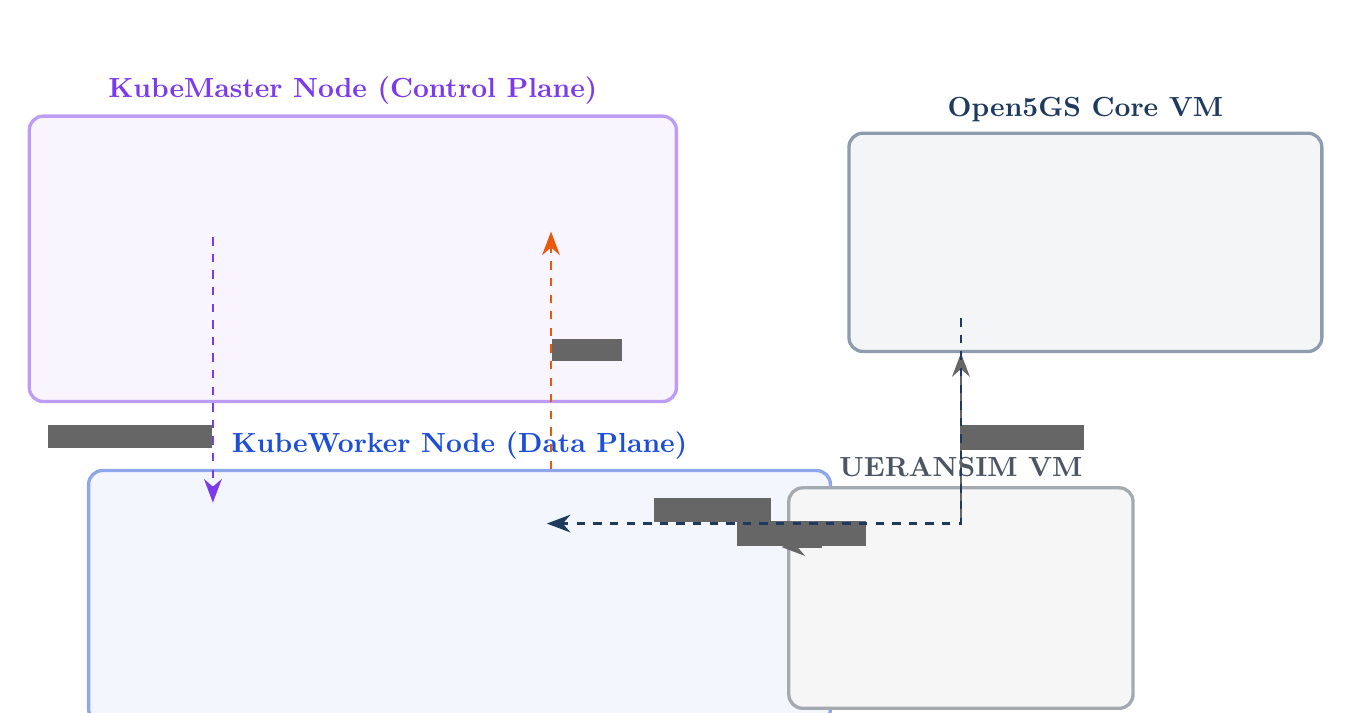
\begin{tikzpicture}[
  node distance=1cm and 1.5cm,
  host/.style={draw, very thick, rounded corners=5pt, inner sep=12pt, fill=#1!5, draw=#1!50},
  vmpod/.style={draw, thick, rounded corners=2pt, fill=#1!20, draw=#1!80, font=\small\bfseries, align=center, inner sep=5pt},
  flow/.style={-{Stealth[length=3mm]}, thick, color=gray!80!black},
  lbl/.style={font=\scriptsize, fill=white, inner sep=1pt, color=gray!80!black}
]

  % KubeMaster Node
  \begin{scope}[local bounding box=master_box]
    \node[vmpod=corch] (agentic) {Agentic Orchestrator\\[0.1cm] \tiny (Observe $\to$ Think $\to$ Act)};
    \node[vmpod=cprom, right=1.2cm of agentic] (prom) {Prometheus \\\& Grafana};
    \node[vmpod=c5g, below=0.6cm of agentic] (llm) {LLM Backend\\(Ollama)};
    \draw[flow, <->] (agentic) -- node[lbl, left]{Inference} (llm);
    \draw[flow, <-] (agentic) -- node[lbl, above]{Metrics} (prom);
  \end{scope}
  \node[host=corch, fit=(master_box)(prom)(llm), label={[font=\bfseries, text=corch]north:KubeMaster Node (Control Plane)}] (master) {};

  % KubeWorker Node
  \begin{scope}[local bounding box=worker_box, shift={(0,-4.5)}]
    \node[vmpod=cembb] (upf1) {UPF-eMBB\\[0.1cm]\tiny (\texttt{tc} enforcement)};
    \node[vmpod=curllc, right=0.5cm of upf1] (upf2) {UPF-URLLC};
    \node[vmpod=cmmtc, right=0.5cm of upf2] (upf3) {UPF-mMTC};
    
    \node[vmpod=cembb, fill=cembb!8!white, below=0.6cm of upf1] (app1) {nginx App};
    \node[vmpod=curllc, fill=curllc!8!white, below=0.6cm of upf2] (app2) {NodeRED App};
    \node[vmpod=cmmtc,  fill=cmmtc!8!white, below=0.6cm of upf3] (app3) {Mosquitto App};

    \draw[flow] (upf1) -- (app1);
    \draw[flow] (upf2) -- (app2);
    \draw[flow] (upf3) -- (app3);
  \end{scope}
  \node[host=cembb, fit=(worker_box)(app3), label={[font=\bfseries, text=cembb]north:KubeWorker Node (Data Plane)}] (worker) {};

  % Open5GS Core VM
  \begin{scope}[local bounding box=core_box, shift={(9.5, 0)}]
    \node[vmpod=c5g, minimum width=2cm] (amf) {AMF};
    \node[vmpod=c5g, right=0.4cm of amf, minimum width=2cm] (nrf) {NRF / NSSF};
    \node[vmpod=c5g, below=0.6cm of amf, minimum width=2cm] (smf) {SMF (x3)};
    \node[vmpod=c5g, right=0.4cm of smf, minimum width=2cm] (udm) {UDM / AUSF};
  \end{scope}
  \node[host=c5g, fit=(core_box)(udm), label={[font=\bfseries, text=c5g]north:Open5GS Core VM}] (core) {};

  % UERANSIM VM
  \begin{scope}[local bounding box=ran_box, shift={(9.5, -4.5)}]
    \node[vmpod=cran, minimum width=3.5cm] (gnb) {gNB Emulator};
    \node[vmpod=cran, fill=cran!8!white, below=0.6cm of gnb, minimum width=3.5cm] (ue) {UEs (3 per slice)};
    \draw[flow, <->] (ue) -- node[lbl, left]{Uu Interface} (gnb);
  \end{scope}
  \node[host=cran, fit=(ran_box)(ue)(gnb), label={[font=\bfseries, text=cran]north:UERANSIM VM}] (ran) {};

  % Inter-host connections
  \draw[flow] (gnb.north) -- node[lbl, right]{N2 (NGAP)} (amf.south |- core.south);
  \draw[flow] (gnb.west) -- node[lbl, above]{N3 (GTP-U)} (upf3.east |- gnb.west);
  
  \draw[flow, dashed, color=corch, thick] (agentic.south) -- node[lbl, left, near end]{SSH QoS Config} (upf1.north);
  \draw[flow, dashed, color=cprom, thick] (worker.north -| prom.south) -- node[lbl, right]{Scrape} (prom.south);
  \draw[flow, dashed, color=c5g, thick] (smf.south) |- node[lbl, above, pos=0.8]{N4 (PFCP)} (upf2.north east);

\end{tikzpicture}}
\caption{Comprehensive Agentic Testbed Architecture, illustrating the physical separation of nodes and the decoupling of the multi-agent control loop from the 5G data plane.}
\label{fig:testbed_arch}
\end{figure}

Figure~\ref{fig:slice_arch} demonstrates the slicing architecture across the three isolated instances.

\begin{figure}[H]
\centering
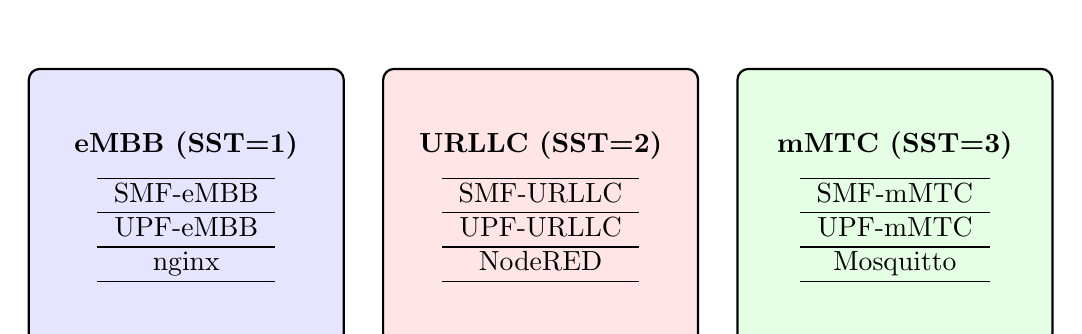
\begin{tikzpicture}[
  slice/.style={draw, rounded corners, thick, minimum width=4cm, minimum height=3.5cm, align=center}
]
\node[slice, fill=blue!10] (embb) at (0,0) {\textbf{eMBB (SST=1)}\\[0.2cm] \begin{tabular}{c} \hline SMF-eMBB \\ \hline UPF-eMBB \\ \hline nginx \\ \hline \end{tabular}};
\node[slice, fill=red!10] (urllc) at (4.5,0) {\textbf{URLLC (SST=2)}\\[0.2cm] \begin{tabular}{c} \hline SMF-URLLC \\ \hline UPF-URLLC \\ \hline NodeRED \\ \hline \end{tabular}};
\node[slice, fill=green!10] (mmtc) at (9,0) {\textbf{mMTC (SST=3)}\\[0.2cm] \begin{tabular}{c} \hline SMF-mMTC \\ \hline UPF-mMTC \\ \hline Mosquitto \\ \hline \end{tabular}};
\end{tikzpicture}
\caption{Slice Architecture showing complete isolation.}
\label{fig:slice_arch}
\end{figure}

Figure~\ref{fig:ue_flow} shows the UE Registration and Slice Selection sequence flow.

\begin{figure}[H]
\centering
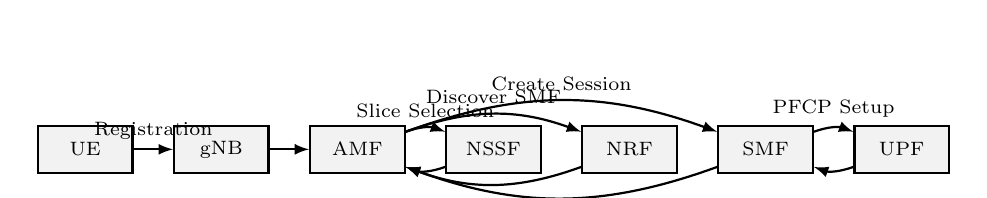
\begin{tikzpicture}[
  agent/.style={draw, thick, minimum width=1.2cm, minimum height=0.6cm, fill=gray!10, font=\scriptsize},
  msg/.style={-latex, thick}
]
\matrix[column sep=0.5cm, row sep=0.8cm] {
\node[agent] (ue) {UE}; & \node[agent] (gnb) {gNB}; & \node[agent] (amf) {AMF}; & \node[agent] (nssf) {NSSF}; & \node[agent] (nrf) {NRF}; & \node[agent] (smf) {SMF}; & \node[agent] (upf) {UPF}; \\
};
\draw[msg] (ue) -- node[above, font=\scriptsize] {Registration} (gnb);
\draw[msg] (gnb) -- (amf);
\draw[msg] (amf) edge[bend left=20] node[above, font=\scriptsize] {Slice Selection} (nssf);
\draw[msg] (nssf) edge[bend left=20] (amf);
\draw[msg] (amf) edge[bend left=20] node[above, font=\scriptsize] {Discover SMF} (nrf);
\draw[msg] (nrf) edge[bend left=20] (amf);
\draw[msg] (amf) edge[bend left=20] node[above, font=\scriptsize] {Create Session} (smf);
\draw[msg] (smf) edge[bend left=20] node[above, font=\scriptsize] {PFCP Setup} (upf);
\draw[msg] (upf) edge[bend left=20] (smf);
\draw[msg] (smf) edge[bend left=20] (amf);
\end{tikzpicture}
\caption{UE Registration \& Slice Selection Flow.}
\label{fig:ue_flow}
\end{figure}

\section{MEC Architecture}

Figure~\ref{fig:mec_locality} proves MEC traffic locality (local breakout).

\begin{figure}[H]
\centering
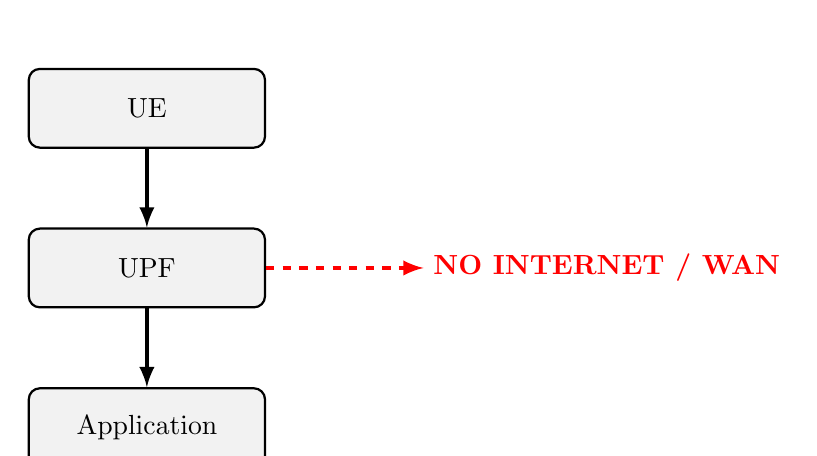
\begin{tikzpicture}[
  box/.style={draw, rounded corners, thick, minimum width=3cm, minimum height=1cm, align=center, fill=gray!10},
  arrow/.style={-latex, thick, line width=1.5pt}
]
\node[box] (ue) {UE};
\node[box, below=1cm of ue] (upf) {UPF};
\node[box, below=1cm of upf] (app) {Application};
\node[right=2cm of upf, font=\bfseries, color=red] (wan) {NO INTERNET / WAN};
\draw[arrow] (ue) -- (upf);
\draw[arrow] (upf) -- (app);
\draw[arrow, red, dashed] (upf) -- (wan);
\end{tikzpicture}
\caption{MEC Traffic Locality with local breakout.}
\label{fig:mec_locality}
\end{figure}

Figure~\ref{fig:k8s_deploy} illustrates the Kubernetes deployment diagram.

\begin{figure}[H]
\centering
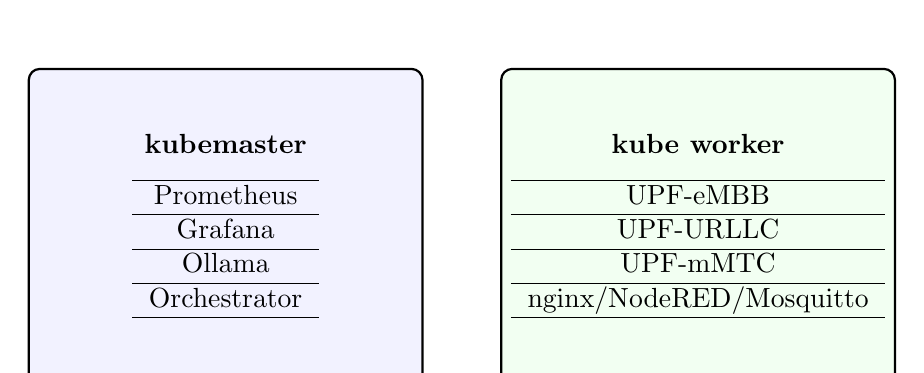
\begin{tikzpicture}[
  nodebox/.style={draw, rounded corners, thick, minimum width=5cm, minimum height=4cm, align=center}
]
\node[nodebox, fill=blue!5] (master) at (0,0) {\textbf{kubemaster}\\[0.3cm] \begin{tabular}{c} \hline Prometheus \\ \hline Grafana \\ \hline Ollama \\ \hline Orchestrator \\ \hline \end{tabular}};
\node[nodebox, fill=green!5] (worker) at (6,0) {\textbf{kube worker}\\[0.3cm] \begin{tabular}{c} \hline UPF-eMBB \\ \hline UPF-URLLC \\ \hline UPF-mMTC \\ \hline nginx/NodeRED/Mosquitto \\ \hline \end{tabular}};
\end{tikzpicture}
\caption{Kubernetes Deployment Diagram.}
\label{fig:k8s_deploy}
\end{figure}

\section{Control Loop}

Figure~\ref{fig:closed_loop} illustrates the Closed Loop QoS Control mechanism.

\begin{figure}[H]
\centering
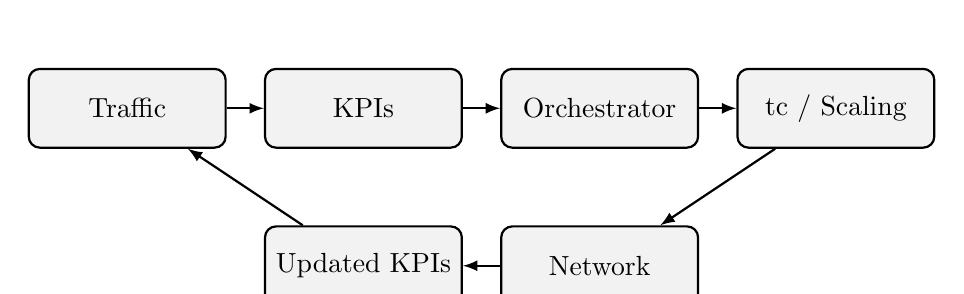
\begin{tikzpicture}[
  box/.style={draw, rounded corners, thick, minimum width=2.5cm, minimum height=1cm, align=center, fill=gray!10},
  arrow/.style={-latex, thick}
]
\node[box] (traffic) at (0,0) {Traffic};
\node[box] (kpis) at (3,0) {KPIs};
\node[box] (orch) at (6,0) {Orchestrator};
\node[box] (tc) at (9,0) {tc / Scaling};
\node[box] (net) at (6,-2) {Network};
\node[box] (ukpis) at (3,-2) {Updated KPIs};

\draw[arrow] (traffic) -- (kpis);
\draw[arrow] (kpis) -- (orch);
\draw[arrow] (orch) -- (tc);
\draw[arrow] (tc) -- (net);
\draw[arrow] (net) -- (ukpis);
\draw[arrow] (ukpis) -- (traffic);
\end{tikzpicture}
\caption{Closed Loop QoS Control.}
\label{fig:closed_loop}
\end{figure}

Figure~\ref{fig:tc_enf} identifies the \texttt{tc} enforcement point at the UPF.

\begin{figure}[H]
\centering
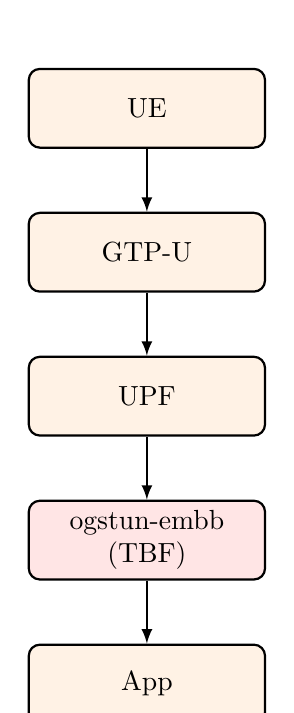
\begin{tikzpicture}[
  box/.style={draw, rounded corners, thick, minimum width=3cm, minimum height=1cm, align=center, fill=orange!10},
  arrow/.style={-latex, thick}
]
\node[box] (ue) {UE};
\node[box, below=0.8cm of ue] (gtp) {GTP-U};
\node[box, below=0.8cm of gtp] (upf) {UPF};
\node[box, below=0.8cm of upf, fill=red!10] (tun) {ogstun-embb\\(TBF)};
\node[box, below=0.8cm of tun] (app) {App};

\draw[arrow] (ue) -- (gtp);
\draw[arrow] (gtp) -- (upf);
\draw[arrow] (upf) -- (tun);
\draw[arrow] (tun) -- (app);
\end{tikzpicture}
\caption{\texttt{tc} Enforcement Point.}
\label{fig:tc_enf}
\end{figure}
\section{Six Research Contributions}
\begin{contribbox}{Project Contributions}
\begin{enumerate}[noitemsep,leftmargin=*]
  \item \textbf{C1 — Autonomous QoS Orchestration Framework}: A cloud-native, closed-loop system that enforces per-slice QoS on live 5G traffic without human intervention.
  \item \textbf{C2 — LangGraph Multi-Agent Architecture}: A stateful five-node agent graph (Observe$\to$Think$\to$Validate$\to$Act$\to$Reflect) coordinating specialised agents.
  \item \textbf{C3 — Chain-of-Thought Network Reasoning}: A mandatory JSON CoT schema requiring \texttt{root\_cause\_assessment} and \texttt{lever\_validity} before any control action.
  \item \textbf{C4 — Wrong-Lever Avoidance Mechanism}: A rolling relative-load metric ($\rho_{\text{eMBB}}$) that prevents erroneous eMBB throttling when eMBB is idle.
  \item \textbf{C5 — Memory-Assisted Decision Making}: A persistent ring-buffer Agent Memory injecting empirical action-outcome history into every LLM prompt.
  \item \textbf{C6 — Comparative Evaluation}: A pre-registered three-scenario behavioral audit comparing Agentic vs.\ Rule-Based controllers on live testbed traffic.
\end{enumerate}
\end{contribbox}

%% ─────────────────────────────────────────────────────────────
\section{Seven-Layer System Architecture}

Figure~\ref{fig:sevenlayer} presents the complete end-to-end architecture across seven logical layers.

\begin{figure}[H]
\centering
\resizebox{\textwidth}{!}{%
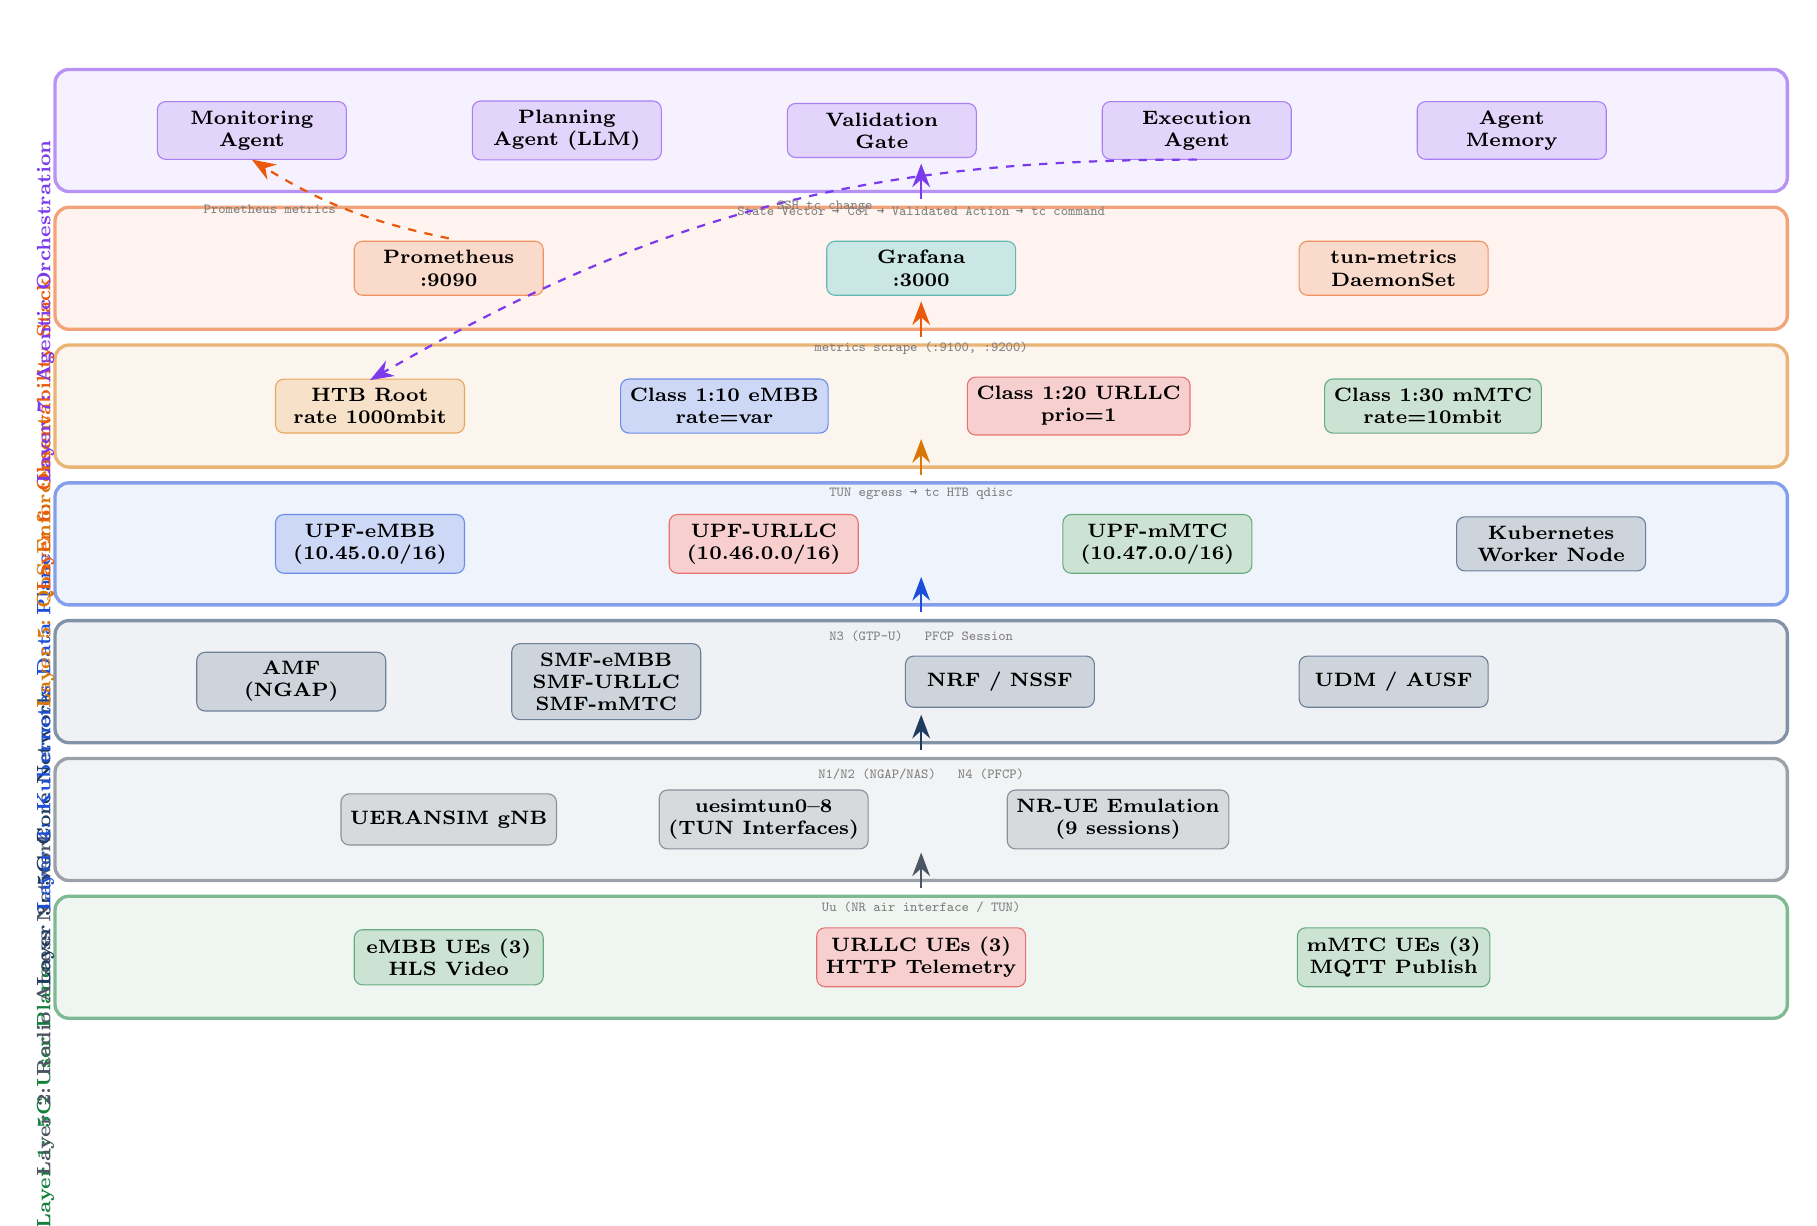
\begin{tikzpicture}[
  lyr/.style={draw, rounded corners=5pt, very thick,
              minimum width=22cm, minimum height=1.55cm,
              fill=#1!7, draw=#1!55},
  pod/.style={draw, rounded corners=3pt, fill=#1!22, draw=#1!65,
              font=\scriptsize\bfseries, minimum width=2.4cm,
              minimum height=0.65cm, align=center},
  ifc/.style={font=\tiny\ttfamily, text=gray},
  arr/.style={-{Stealth[length=3mm]}, thick, #1},
  lbl/.style={font=\bfseries\scriptsize, rotate=90, text=#1}
]
%% ── Layer backgrounds (bottom=L1, top=L7)
\foreach \i/\col/\name in {
  0/cmmtc/{Layer 1: 5G User Plane},
  1/cran/{Layer 2: Radio Access Network},
  2/c5g/{Layer 3: 5G Core Network},
  3/cembb/{Layer 4: Kubernetes Data Plane},
  4/cqos/{Layer 5: QoS Enforcement},
  5/cprom/{Layer 6: Observability Stack},
  6/corch/{Layer 7: Agentic Orchestration}
}{
  \node[lyr=\col] (L\i) at (11, \i*1.75+0.87) {};
  \node[\col, font=\bfseries\scriptsize, left=0.1cm of L\i.west, rotate=90] {\name};
}

%% ── L1: User Plane
\node[pod=cmmtc] at (5,  0.87) {eMBB UEs (3)\\HLS Video};
\node[pod=curllc] at (11, 0.87) {URLLC UEs (3)\\HTTP Telemetry};
\node[pod=cmmtc]  at (17, 0.87) {mMTC UEs (3)\\MQTT Publish};

%% ── L2: RAN
\node[pod=cran] at (5,  2.62) {UERANSIM gNB};
\node[pod=cran] at (9,  2.62) {uesimtun0--8\\(TUN Interfaces)};
\node[pod=cran] at (13.5, 2.62) {NR-UE Emulation\\(9 sessions)};
\node[ifc] at (11, 1.5) {Uu (NR air interface / TUN)};

%% ── L3: 5G Core
\node[pod=c5g] at (3,  4.37) {AMF\\(NGAP)};
\node[pod=c5g] at (7,  4.37) {SMF-eMBB\\SMF-URLLC\\SMF-mMTC};
\node[pod=c5g] at (12, 4.37) {NRF / NSSF};
\node[pod=c5g] at (17, 4.37) {UDM / AUSF};
\node[ifc] at (11, 3.2) {N1/N2 (NGAP/NAS) \quad N4 (PFCP)};

%% ── L4: K8s Data Plane
\node[pod=cembb]  at (4,   6.12) {UPF-eMBB\\(10.45.0.0/16)};
\node[pod=curllc] at (9,   6.12) {UPF-URLLC\\(10.46.0.0/16)};
\node[pod=cmmtc]  at (14,  6.12) {UPF-mMTC\\(10.47.0.0/16)};
\node[pod=c5g]    at (19,  6.12) {Kubernetes\\Worker Node};
\node[ifc] at (11, 4.95) {N3 (GTP-U) \quad PFCP Session};

%% ── L5: QoS Enforcement
\node[pod=cqos] at (4,   7.87) {HTB Root\\rate 1000mbit};
\node[pod=cembb] at (8.5,7.87) {Class 1:10 eMBB\\rate=\textbf{var}};
\node[pod=curllc] at (13,7.87) {Class 1:20 URLLC\\prio=1};
\node[pod=cmmtc] at (17.5,7.87){Class 1:30 mMTC\\rate=10mbit};
\node[ifc] at (11, 6.75) {TUN egress → tc HTB qdisc};

%% ── L6: Observability
\node[pod=cprom] at (5,  9.62) {Prometheus\\:9090};
\node[pod=cgraf]  at (11, 9.62) {Grafana\\:3000};
\node[pod=cprom]  at (17, 9.62) {tun-metrics\\DaemonSet};
\node[ifc] at (11, 8.6) {metrics scrape (:9100, :9200)};

%% ── L7: Orchestration
\node[pod=corch] at (2.5,11.37) {Monitoring\\Agent};
\node[pod=corch] at (6.5, 11.37) {Planning\\Agent (LLM)};
\node[pod=corch] at (10.5,11.37) {Validation\\Gate};
\node[pod=corch] at (14.5,11.37) {Execution\\Agent};
\node[pod=corch] at (18.5,11.37) {Agent\\Memory};
\node[ifc] at (11, 10.35) {State Vector → CoT → Validated Action → tc command};

%% ── Vertical interface arrows (between layer centers)
\draw[arr=cran]  (11,1.75) -- (11,2.2);
\draw[arr=c5g]   (11,3.5)  -- (11,3.95);
\draw[arr=cembb] (11,5.25) -- (11,5.7);
\draw[arr=cqos]  (11,7.0)  -- (11,7.45);
\draw[arr=cprom] (11,8.75) -- (11,9.2);
\draw[arr=corch] (11,10.5) -- (11,10.95);

%% ── Feedback: Orchestrator → QoS (SSH tc command)
\draw[arr=corch, bend right=15, dashed, thick]
  (14.5,11.0) to node[right, ifc, pos=0.5]{SSH tc change} (4,8.2);

%% ── Observability → Orchestrator
\draw[arr=cprom, bend left=10, dashed]
  (5,10.0) to node[left, ifc, pos=0.5]{Prometheus metrics} (2.5,11.0);

\end{tikzpicture}}
\caption{Seven-Layer End-to-End System Architecture. Solid arrows denote data-plane flows; dashed arrows denote control and observability flows.}
\label{fig:sevenlayer}
\end{figure}

%% ─────────────────────────────────────────────────────────────
\section{Agentic Orchestration Framework}

\begin{figure}[H]
\centering
\resizebox{\textwidth}{!}{%
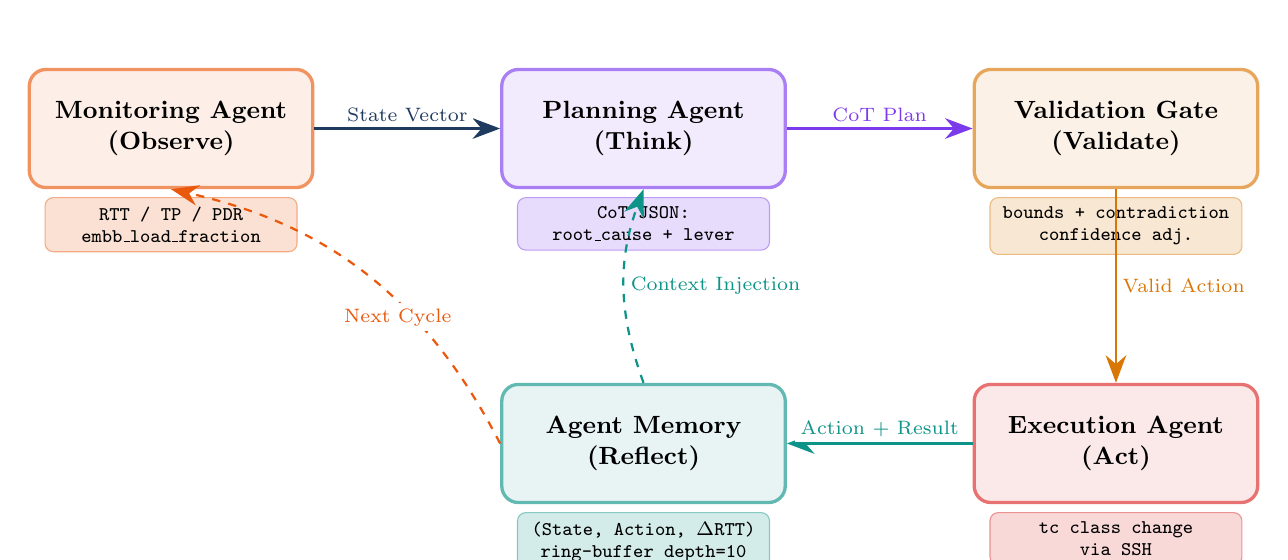
\begin{tikzpicture}[
  agent/.style={draw, rounded corners=6pt, fill=#1!10, draw=#1!65,
                very thick, minimum width=3.6cm, minimum height=1.5cm,
                align=center, font=\small\bfseries},
  sub/.style={draw, rounded corners=3pt, fill=#1!18, draw=#1!50,
              font=\scriptsize\ttfamily, minimum width=3.2cm,
              minimum height=0.55cm, align=center},
  arr/.style={-{Stealth[length=3.5mm]}, thick, #1},
  lbl/.style={font=\scriptsize, fill=white, inner sep=2pt, align=center}
]

%% Agents
\node[agent=cprom]  (mon)  at (0,0)    {Monitoring Agent\\(Observe)};
\node[agent=corch]  (plan) at (6,0)    {Planning Agent\\(Think)};
\node[agent=cqos]   (val)  at (12,0)   {Validation Gate\\(Validate)};
\node[agent=curllc] (exec) at (12,-4)  {Execution Agent\\(Act)};
\node[agent=cgraf]  (mem)  at (6,-4)   {Agent Memory\\(Reflect)};

%% Sub-labels
\node[sub=cprom, below=0.1cm of mon]  {RTT / TP / PDR\\embb\_load\_fraction};
\node[sub=corch, below=0.1cm of plan] {CoT JSON:\\root\_cause + lever};
\node[sub=cqos,  below=0.1cm of val]  {bounds + contradiction\\confidence adj.};
\node[sub=curllc,below=0.1cm of exec] {\texttt{tc class change}\\via SSH};
\node[sub=cgraf, below=0.1cm of mem]  {(State, Action, $\Delta$RTT)\\ring-buffer depth=10};

%% Main pipeline
\draw[arr=c5g]   (mon)  -- node[lbl, above]{State Vector}   (plan);
\draw[arr=corch] (plan) -- node[lbl, above]{CoT Plan}        (val);
\draw[arr=cqos]  (val)  -- node[lbl, right]{Valid Action}    (exec);
\draw[arr=cgraf] (exec) -- node[lbl, above]{Action + Result} (mem);

%% Memory ↔ Planner feedback
\draw[arr=cgraf, dashed, bend left=20]
  (mem.north) to node[lbl, right]{Context Injection} (plan.south);

%% Monitor ← memory update
\draw[arr=cprom, dashed, bend right=25]
  (mem.west) to node[lbl, below, pos=0.4]{Next Cycle} (mon.south);

\end{tikzpicture}}
\caption{LangGraph Multi-Agent Orchestration Pipeline (Contribution C2). Each node is a specialised agent; dashed arrows represent cross-cycle feedback.}
\label{fig:langgraph_pipeline}
\end{figure}

%% ─────────────────────────────────────────────────────────────
\section{Individual Agent Architecture}

\subsection{Monitoring Agent}
\begin{figure}[H]
\centering
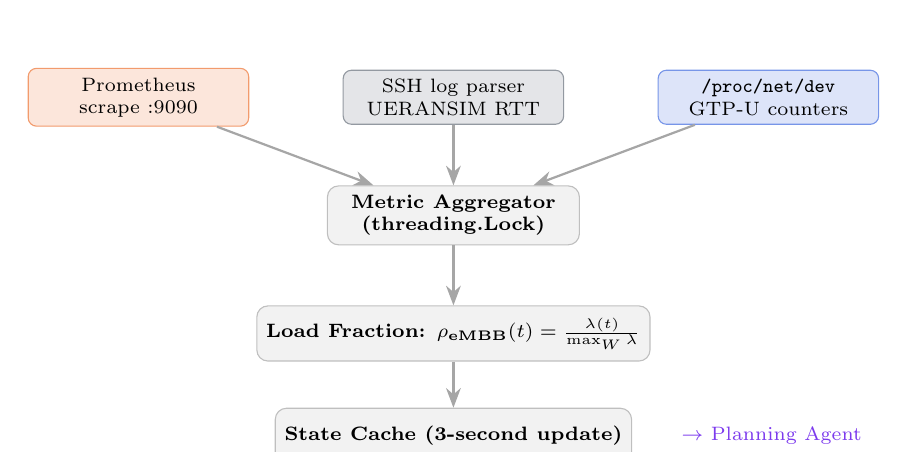
\begin{tikzpicture}[
  src/.style={draw, rounded corners=3pt, fill=#1!15, draw=#1!60,
              font=\scriptsize, minimum width=2.8cm, minimum height=0.6cm, align=center},
  box/.style={draw, rounded corners=4pt, fill=gray!10, draw=gray!50,
              font=\scriptsize\bfseries, minimum width=3.2cm, minimum height=0.7cm, align=center},
  arr/.style={-{Stealth[length=2.5mm]}, thick, gray!70}
]
\node[src=cprom] (prom)  at (0,4)   {Prometheus\\scrape :9090};
\node[src=cran]  (ssh)   at (4,4)   {SSH log parser\\UERANSIM RTT};
\node[src=cembb] (proc)  at (8,4)   {\texttt{/proc/net/dev}\\GTP-U counters};

\node[box] (agg) at (4,2.5) {Metric Aggregator\\(threading.Lock)};
\node[box] (frac) at (4,1)  {Load Fraction: $\rho_{\text{eMBB}}(t) = \tfrac{\lambda(t)}{\max_{W}\lambda}$};
\node[box] (cache) at (4,-0.3) {State Cache (3-second update)};

\draw[arr] (prom)  -- (agg);
\draw[arr] (ssh)   -- (agg);
\draw[arr] (proc)  -- (agg);
\draw[arr] (agg)   -- (frac);
\draw[arr] (frac)  -- (cache);
\node[font=\scriptsize, right=0.5cm of cache, text=corch]
  {$\rightarrow$ Planning Agent};
\end{tikzpicture}
\caption{Monitoring Agent Architecture (Contribution C4). Three input collectors feed an aggregator; the derived load-fraction metric is written to the thread-safe state cache.}
\label{fig:mon_agent}
\end{figure}

\subsection{Planning Agent}
\begin{figure}[H]
\centering
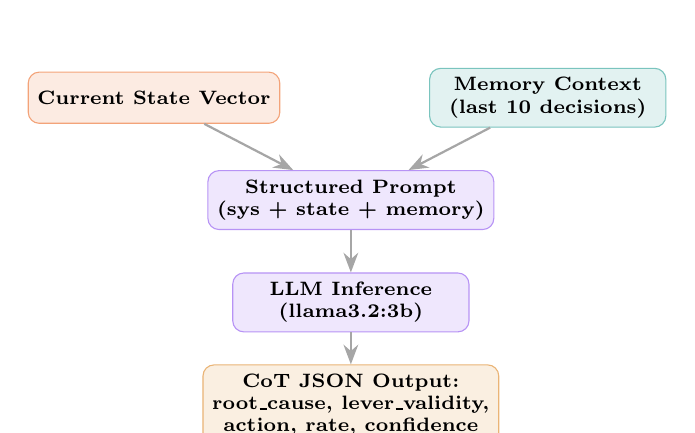
\begin{tikzpicture}[
  box/.style={draw, rounded corners=4pt, fill=#1!12, draw=#1!55,
              font=\scriptsize\bfseries, minimum width=3.0cm, minimum height=0.65cm, align=center},
  arr/.style={-{Stealth[length=2.5mm]}, thick, gray!70},
  lbl/.style={font=\scriptsize, text=gray}
]
\node[box=cprom] (state) at (0,3.5)   {Current State Vector};
\node[box=cgraf]  (mem)  at (5,3.5)   {Memory Context\\(last 10 decisions)};
\node[box=corch] (prompt) at (2.5,2.2) {Structured Prompt\\(sys + state + memory)};
\node[box=corch] (llm)   at (2.5,0.9) {LLM Inference\\(llama3.2:3b)};
\node[box=cqos]  (cot)   at (2.5,-0.4){CoT JSON Output:\\root\_cause, lever\_validity,\\action, rate, confidence};

\draw[arr] (state) -- (prompt);
\draw[arr] (mem)   -- (prompt);
\draw[arr] (prompt) -- (llm);
\draw[arr] (llm)   -- (cot);
\end{tikzpicture}
\caption{Planning Agent Architecture (Contributions C3, C5). State and memory are injected into a structured prompt; the LLM generates a mandatory CoT schema.}
\label{fig:plan_agent}
\end{figure}

\subsection{Validation Gate}
\begin{figure}[H]
\centering
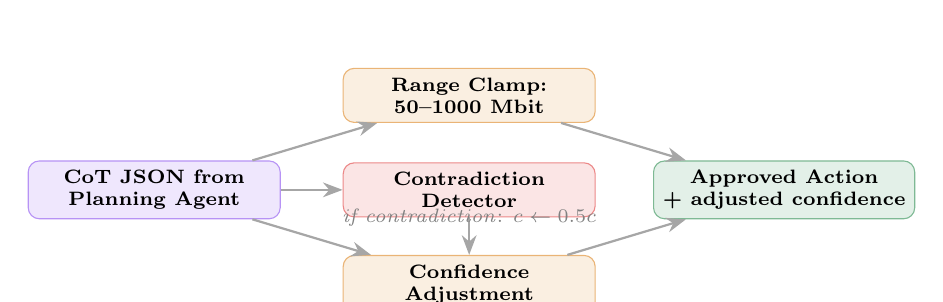
\begin{tikzpicture}[
  box/.style={draw, rounded corners=4pt, fill=#1!12, draw=#1!55,
              font=\scriptsize\bfseries, minimum width=3.2cm, minimum height=0.65cm, align=center},
  arr/.style={-{Stealth[length=2.5mm]}, thick, gray!70},
  lbl/.style={font=\scriptsize, text=gray}
]
\node[box=corch] (in)   at (0,0)    {CoT JSON from\\Planning Agent};
\node[box=cqos]  (rng)  at (4,1.2)  {Range Clamp:\\50–1000 Mbit};
\node[box=curllc](cdet) at (4,0)    {Contradiction\\Detector};
\node[box=cqos]  (conf) at (4,-1.2) {Confidence\\Adjustment};
\node[box=cmmtc] (out)  at (8,0)    {Approved Action\\+ adjusted confidence};

\draw[arr] (in)  -- (rng);
\draw[arr] (in)  -- (cdet);
\draw[arr] (in)  -- (conf);
\draw[arr] (rng)  -- (out);
\draw[arr] (cdet) -- node[lbl,above]{\textit{if contradiction}: $c \gets 0.5c$} (conf);
\draw[arr] (conf) -- (out);
\end{tikzpicture}
\caption{Validation Gate Architecture (Contribution C4). Contradiction detection catches logical inconsistencies between the \texttt{root\_cause\_assessment} and the proposed action.}
\label{fig:val_gate}
\end{figure}

%% ─────────────────────────────────────────────────────────────
\section{Mathematical Foundations}

Table~\ref{tab:notation} defines the notation used throughout this report.

\begin{table}[H]
\centering
\caption{Mathematical Notation}
\label{tab:notation}
\begin{tabularx}{\textwidth}{llX}
\toprule
\textbf{Symbol} & \textbf{Unit} & \textbf{Definition} \\
\midrule
$\rho_{\text{eMBB}}(t)$ & — & eMBB relative load fraction at time $t$ \\
$\lambda(t)$  & pkt/s  & eMBB packet rate at time $t$ \\
$W$           & cycles & Rolling window size (default: 8) \\
$R(t)$        & ms     & URLLC RTT$_{99}$ at time $t$ \\
$\theta$      & ms     & URLLC SLA threshold (20\,ms) \\
$r(t)$        & Mbit/s & eMBB \texttt{tc} rate cap at time $t$ \\
$r_{\max}$    & Mbit/s & Maximum eMBB rate (1000\,Mbit) \\
$T_{\text{rec}}$ & s   & SLA recovery time \\
$C_{\text{sla}}$ & —   & SLA compliance ratio \\
$\eta_{\text{act}}$ & — & Action efficiency \\
$N_T$         & —      & Total monitoring cycles \\
$N_V$         & —      & Cycles with SLA violation ($R > \theta$) \\
\bottomrule
\end{tabularx}
\end{table}

\subsection{eMBB Load Fraction}

The eMBB relative load fraction is the central metric enabling Contribution C4. Unlike absolute throughput, it is invariant to traffic profile differences:

\begin{equation}
\rho_{\text{eMBB}}(t) = \frac{\lambda(t)}{\displaystyle\max_{t' \in [t-W\Delta, t]} \lambda(t')}
\label{eq:load_frac}
\end{equation}

where $\Delta = 3$\,s is the monitoring interval and $W = 8$ is the rolling window. $\rho_{\text{eMBB}} \in [0, 1]$; a value $< 0.2$ indicates a low-activity slice that should not be throttled regardless of RTT.

\subsection{SLA Compliance Ratio}

\begin{equation}
C_{\text{sla}} = 1 - \frac{N_V}{N_T} = \frac{\#\{t : R(t) \leq \theta\}}{N_T}
\label{eq:sla_comp}
\end{equation}

\subsection{Recovery Time}

Recovery time is the interval from the first SLA breach until the RTT falls back below $\theta$:

\begin{equation}
T_{\text{rec}} = t_{\text{clear}} - t_{\text{breach}}, \quad t_{\text{clear}} = \min\{t > t_{\text{breach}} : R(t) \leq \theta\}
\label{eq:trec}
\end{equation}

\subsection{Throughput Preservation Ratio}

\begin{equation}
\text{TP} = 1 - \frac{\displaystyle\sum_{t: r(t) < r_{\max}} (r_{\max} - r(t)) \cdot \Delta}{\displaystyle r_{\max} \cdot N_T \cdot \Delta}
\label{eq:tp}
\end{equation}

\subsection{Action Efficiency}

The fraction of throttle actions that followed a genuine SLA violation or rising trend:

\begin{equation}
\eta_{\text{act}} = \frac{\#\{\text{throttle}: R > \theta \text{ or trend rising}\}}{\#\{\text{throttle actions}\}}
\label{eq:eff}
\end{equation}

%% ─────────────────────────────────────────────────────────────
\section{Control Loop State Transition Diagram}

\begin{figure}[H]
\centering
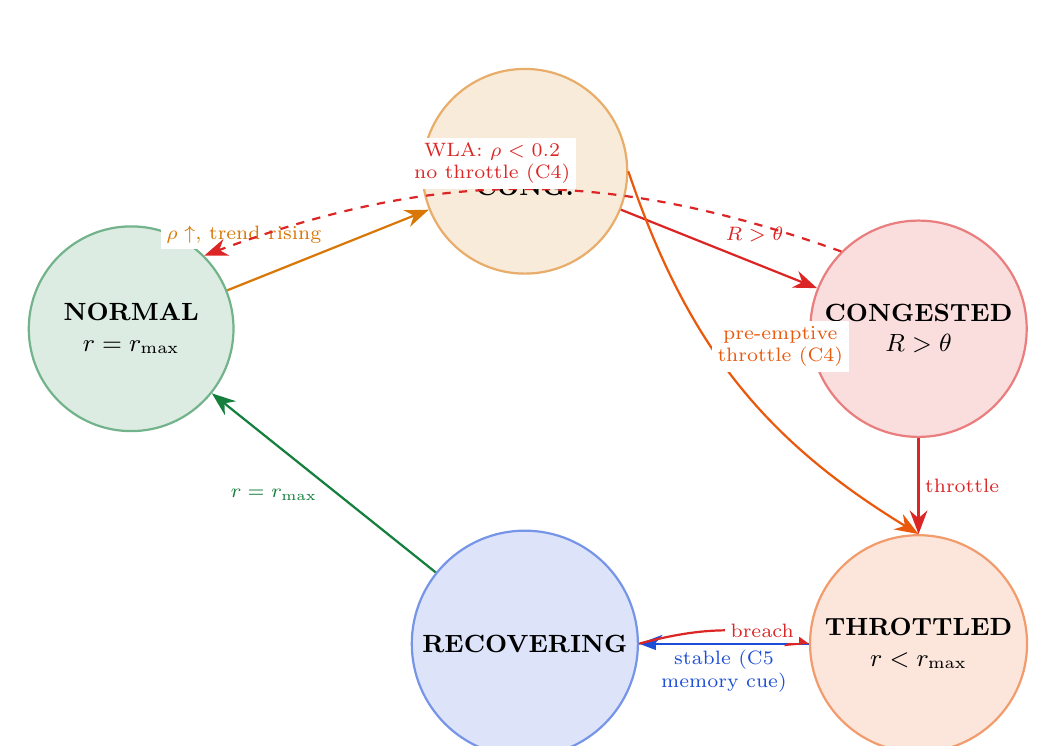
\begin{tikzpicture}[
  state/.style={draw, circle, minimum size=2.6cm, font=\small\bfseries,
                align=center, thick, fill=#1!15, draw=#1!60},
  arr/.style={-{Stealth[length=3mm]}, thick},
  lbl/.style={font=\scriptsize, align=center, fill=white, inner sep=2pt}
]
\node[state=cmmtc]  (N)  at (0,0)    {NORMAL\\$r=r_{\max}$};
\node[state=cqos]   (P)  at (5,2)    {PRE-\\CONG.};
\node[state=curllc] (C)  at (10,0)   {CONGESTED\\$R>\theta$};
\node[state=cprom]  (T)  at (10,-4)  {THROTTLED\\$r<r_{\max}$};
\node[state=cembb]  (R)  at (5,-4)   {RECOVERING};

\draw[arr,cqos]  (N) -- node[lbl,above left]{$\rho\uparrow$, trend rising} (P);
\draw[arr,curllc](P) -- node[lbl,above right]{$R>\theta$} (C);
\draw[arr,cprom, bend right=20] (P.east) to node[lbl,right,pos=0.4]{pre-emptive\\throttle (C4)} (T.north);
\draw[arr,curllc](C) -- node[lbl,right]{throttle} (T);
\draw[arr,cembb] (T) -- node[lbl,below]{stable (C5\\memory cue)} (R);
\draw[arr,cmmtc] (R) -- node[lbl,below left]{$r=r_{\max}$} (N);
\draw[arr,curllc,bend right=20,dashed](C.north west) to node[lbl,above,pos=0.55]{WLA: $\rho<0.2$\\no throttle (C4)} (N.north east);
\draw[arr,curllc,bend left=15](R.east) to node[lbl,right]{breach} (T.west);
\end{tikzpicture}
\caption{Orchestrator Control Loop State Machine. WLA = Wrong-Lever Avoidance (C4). The dashed path is structurally impossible in rule-based systems.}
\label{fig:fsm}
\end{figure}

%% ch_algorithms.tex — Algorithm Design
\chapter{ALGORITHM DESIGN}

This chapter presents the six core algorithms that constitute the Agentic Orchestrator. Each algorithm is formally defined with pseudocode, input/output specifications, and complexity analysis.

\section{Orchestrator Design Diagrams}

Figure~\ref{fig:rule_based} shows the Rule-Based Workflow.

\begin{figure}[H]
\centering
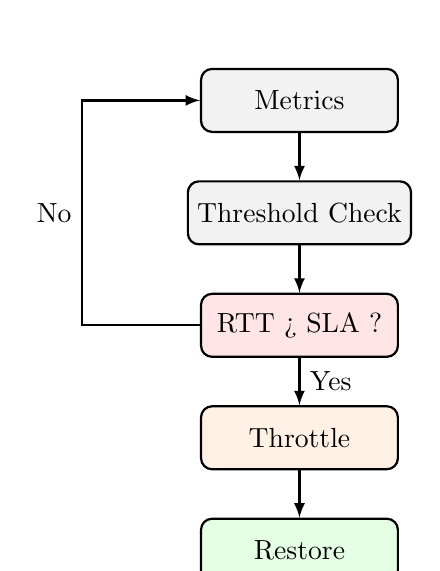
\begin{tikzpicture}[
  box/.style={draw, rounded corners, thick, minimum width=2.5cm, minimum height=0.8cm, align=center, fill=gray!10},
  arrow/.style={-latex, thick}
]
\node[box] (metrics) {Metrics};
\node[box, below=0.6cm of metrics] (thresh) {Threshold Check};
\node[box, below=0.6cm of thresh, fill=red!10] (cond) {RTT > SLA ?};
\node[box, below=0.6cm of cond, fill=orange!10] (throttle) {Throttle};
\node[box, below=0.6cm of throttle, fill=green!10] (restore) {Restore};

\draw[arrow] (metrics) -- (thresh);
\draw[arrow] (thresh) -- (cond);
\draw[arrow] (cond) -- node[right]{Yes} (throttle);
\draw[arrow] (throttle) -- (restore);
\draw[arrow] (cond.west) -- +(-1.5,0) |- node[left, pos=0.25]{No} (metrics.west);
\end{tikzpicture}
\caption{Rule-Based Workflow.}
\label{fig:rule_based}
\end{figure}

Figure~\ref{fig:agentic_flow} presents the Agentic Workflow.

\begin{figure}[H]
\centering
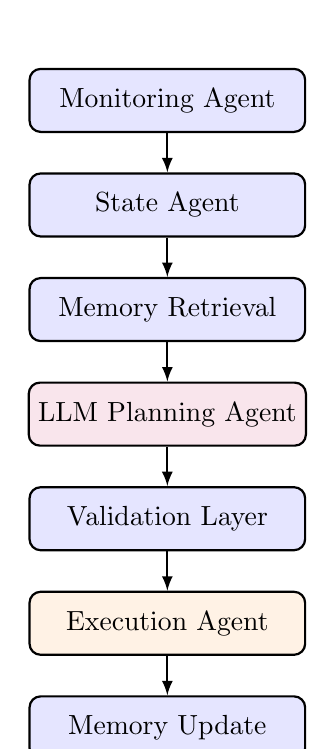
\begin{tikzpicture}[
  box/.style={draw, rounded corners, thick, minimum width=3.5cm, minimum height=0.8cm, align=center, fill=blue!10},
  arrow/.style={-latex, thick}
]
\node[box] (mon) {Monitoring Agent};
\node[box, below=0.5cm of mon] (state) {State Agent};
\node[box, below=0.5cm of state] (mem) {Memory Retrieval};
\node[box, below=0.5cm of mem, fill=purple!10] (llm) {LLM Planning Agent};
\node[box, below=0.5cm of llm] (val) {Validation Layer};
\node[box, below=0.5cm of val, fill=orange!10] (exec) {Execution Agent};
\node[box, below=0.5cm of exec] (memup) {Memory Update};

\draw[arrow] (mon) -- (state);
\draw[arrow] (state) -- (mem);
\draw[arrow] (mem) -- (llm);
\draw[arrow] (llm) -- (val);
\draw[arrow] (val) -- (exec);
\draw[arrow] (exec) -- (memup);
\end{tikzpicture}
\caption{Agentic Workflow.}
\label{fig:agentic_flow}
\end{figure}

Figure~\ref{fig:c345_framework} illustrates the integration of the C3, C4, and C5 frameworks.

\begin{figure}[H]
\centering
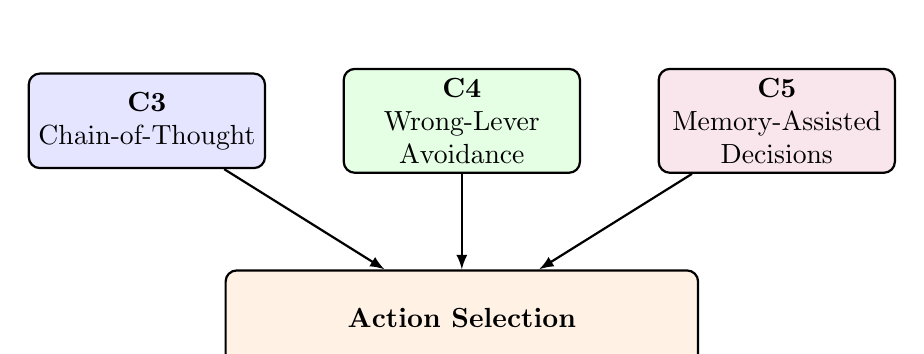
\begin{tikzpicture}[
  box/.style={draw, rounded corners, thick, minimum width=3cm, minimum height=1.2cm, align=center, fill=gray!10},
  arrow/.style={-latex, thick}
]
\node[box, fill=blue!10] (c3) at (0,2) {\textbf{C3}\\Chain-of-Thought};
\node[box, fill=green!10] (c4) at (4,2) {\textbf{C4}\\Wrong-Lever\\Avoidance};
\node[box, fill=purple!10] (c5) at (8,2) {\textbf{C5}\\Memory-Assisted\\Decisions};
\node[box, fill=orange!10, minimum width=6cm] (action) at (4,-0.5) {\textbf{Action Selection}};

\draw[arrow] (c3) -- (action);
\draw[arrow] (c4) -- (action);
\draw[arrow] (c5) -- (action);
\end{tikzpicture}
\caption{C3/C4/C5 Framework contributing to action selection.}
\label{fig:c345_framework}
\end{figure}

%% ─────────────────────────────────────────────────────────────
\section{Algorithm 1: Monitoring and State Collection}

Algorithm~\ref{alg:monitor} describes the decoupled monitoring thread that runs at a fixed 3-second interval independent of LLM inference.

\begin{algorithm}[H]
\caption{Monitoring Agent: Decoupled State Collection}
\label{alg:monitor}
\begin{algorithmic}[1]
\Require Monitoring interval $\Delta = 3\,\text{s}$, SSH credentials, Prometheus endpoint
\Ensure Updated thread-safe state cache $\mathcal{S}$

\While{orchestrator active}
  \State $t_0 \gets \text{time()}$

  \State \textbf{// Channel 1: URLLC RTT via SSH log parse}
  \State $R \gets \text{SSH.exec}(\texttt{"tail -1 /tmp/mec-clients/urllc-*.log"})$
  \State $R \gets \text{parseRTT}(R)$ \Comment{extract $\text{RTT}_{99}$ in ms}

  \State \textbf{// Channel 2: eMBB throughput from /proc/net/dev}
  \State $B_{\text{tx}}, B_{\text{rx}} \gets \text{readProcNetDev}(\texttt{uesimtun1})$
  \State $\lambda_{\text{bps}} \gets (B_{\text{tx}} - B_{\text{tx,prev}}) / \Delta \times 8$
  \State $\lambda_{\text{pkt}} \gets (\text{pkt}_{\text{tx}} - \text{pkt}_{\text{prev}}) / \Delta$

  \State \textbf{// Channel 3: mMTC PDR from MQTT log}
  \State $N_{\text{pub}}, N_{\text{ok}} \gets \text{parseMQTTLog}()$
  \State $\text{PDR} \gets N_{\text{ok}} / N_{\text{pub}}$ \textbf{ if } $N_{\text{pub}} > 0$ \textbf{ else } $1.0$

  \State \textbf{// Derived metrics}
  \State $\rho_{\text{eMBB}} \gets \text{computeLoadFraction}(\lambda_{\text{pkt}})$ \Comment{Algorithm~\ref{alg:loadfrac}}
  \State $d \gets \text{countDeadTunnels}()$

  \State \textbf{// Atomic state cache write}
  \State $\mathcal{S}.\text{acquire}()$
  \State $\mathcal{S} \gets \{R,\, \lambda_{\text{bps}},\, \lambda_{\text{pkt}},\, \rho_{\text{eMBB}},\, \text{PDR},\, d\}$
  \State $\mathcal{S}.\text{release}()$

  \State $\text{sleep}(\Delta - (\text{time}() - t_0))$
\EndWhile
\end{algorithmic}
\end{algorithm}

\textbf{Complexity:} $O(1)$ per cycle. SSH and file I/O dominate; total wall time $\approx 200$\,ms per cycle, leaving $\approx 2.8$\,s idle.

%% ─────────────────────────────────────────────────────────────
\section{Algorithm 2: eMBB Load Fraction Computation}

\begin{algorithm}[H]
\caption{eMBB Load Fraction with Sliding Window}
\label{alg:loadfrac}
\begin{algorithmic}[1]
\Require Packet rate $\lambda(t)$, window $W = 8$, history $\mathcal{H}$ (deque, maxlen $W$)
\Ensure $\rho_{\text{eMBB}}(t) \in [0,1]$ or \texttt{None}

\State $\mathcal{H}.\text{append}(\lambda(t))$
\If{$|\mathcal{H}| < \lceil W/2 \rceil$} \Comment{insufficient history}
  \Return \texttt{None}
\EndIf
\State $\lambda_{\max} \gets \max(\mathcal{H})$
\If{$\lambda_{\max} = 0$}
  \Return $0.0$ \Comment{slice is truly idle}
\EndIf
\Return $\lambda(t) / \lambda_{\max}$
\end{algorithmic}
\end{algorithm}

\textbf{Mathematical Formulation:} As defined in Eq.~\ref{eq:load_frac}, $\rho_{\text{eMBB}}$ normalises the current packet rate against the peak observed over the last $W$ cycles:
\[
  \rho_{\text{eMBB}}(t) = \frac{\lambda(t)}{\max_{k=0}^{W-1} \lambda(t - k\Delta)}
\]

\textbf{Why relative load is superior to absolute throughput:} An absolute threshold (e.g., throttle when eMBB $> 200$\,Mbps) will incorrectly trigger when the application itself is transmitting at 200\,Mbps by design. The relative metric is invariant to application-layer traffic profiles; only genuine burst anomalies ($\rho > 0.9$) drive orchestration decisions.

\textbf{Example:} $\mathcal{H} = [50, 120, 180, 220, 210, 190, 200, 215]$\,pkt/s, $\lambda(t) = 215$. Then $\lambda_{\max} = 220$, $\rho = 215/220 = 0.977$ — \textit{high load}: throttling is warranted.

\textbf{Sliding Window Complexity:} $O(W)$ per cycle for $\max$; $O(1)$ deque append.

%% ─────────────────────────────────────────────────────────────
\section{Algorithm 3: Agentic Planning (Chain-of-Thought)}

\begin{algorithm}[H]
\caption{Planning Agent: CoT-Enforced Action Selection}
\label{alg:plan}
\begin{algorithmic}[1]
\Require State $\mathcal{S}$, Agent Memory $\mathcal{M}$ (last $K=10$ entries)
\Ensure $\{\text{root\_cause},\, \text{lever\_validity},\, \text{action},\, r',\, c\}$

\State $\pi \gets \text{buildSystemPrompt}()$ \Comment{forbids thresholds, mandates CoT schema}
\State $\mu \gets \text{summariseMemory}(\mathcal{M})$ \Comment{last $K$ (action, $\Delta R$) pairs}
\State $\sigma \gets \text{formatStateVector}(\mathcal{S})$ \Comment{RTT, $\rho$, trend, stable\_for, \ldots}
\State $\text{prompt} \gets \pi \oplus \sigma \oplus \mu$

\State $\text{raw} \gets \text{LLM.generate}(\text{prompt},\, \texttt{format=json},\, \texttt{timeout}=60)$

\If{$\text{raw} = \emptyset$} \Comment{timeout}
  \Return $\text{RuleBasedFallback}(\mathcal{S})$ \Comment{Algorithm~\ref{alg:loop}}
\EndIf

\State $\text{cot} \gets \text{parseJSON}(\text{raw})$
\State \textbf{assert} \texttt{root\_cause} $\neq \emptyset$ \textbf{ and } \texttt{lever\_validity} $\neq \emptyset$
\State $r' \gets \text{int}(\text{cot.new\_rate\_mbit})$ \textbf{ or } $r_{\max}$
\State $c \gets \text{float}(\text{cot.confidence})$

\Return $\{\text{cot.root\_cause},\, \text{cot.lever\_validity},\, \text{cot.action},\, r',\, c\}$
\end{algorithmic}
\end{algorithm}

%% ─────────────────────────────────────────────────────────────
\section{Algorithm 4: Validation and Safety Gate}

\begin{algorithm}[H]
\caption{Validation Gate: Safety and Contradiction Detection}
\label{alg:validate}
\begin{algorithmic}[1]
\Require CoT output $\{a, r', c, \text{root\_cause}\}$, bounds $[r_{\min}, r_{\max}]$
\Ensure Safe action $a^*$, adjusted confidence $c^*$

\State \textbf{// Range clamp}
\State $r^* \gets \max(r_{\min},\, \min(r', r_{\max}))$

\State \textbf{// Contradiction detection (Contribution C4)}
\State $\mathcal{K} \gets \{$\textit{"low load", "not the cause", "nearly idle", "not embb"}$\}$
\If{$a = \texttt{throttle\_embb}$ \textbf{ and } $\exists k \in \mathcal{K} : k \in \text{root\_cause}$}
  \State $c^* \gets 0.5 \times c$ \Comment{penalise contradictory reasoning}
  \State $\log.\text{warning}(\texttt{"Contradiction detected"})$
\Else
  \State $c^* \gets c$
\EndIf

\State \textbf{// Dead-tunnel guard}
\If{$\mathcal{S}.\text{dead\_tunnels} = 3$} \Comment{all URLLC tunnels dead}
  \Return $\{\texttt{no\_action},\, r_{\max},\, 0.0\}$ \Comment{monitoring unreliable}
\EndIf

\State \textbf{// Redundant-action guard}
\If{$a = \texttt{throttle\_embb}$ \textbf{ and } $r^* = r_{\text{current}}$}
  \Return $\{\texttt{no\_action},\, r_{\text{current}},\, c^*\}$
\EndIf

\Return $\{a,\, r^*,\, c^*\}$
\end{algorithmic}
\end{algorithm}

%% ─────────────────────────────────────────────────────────────
\section{Algorithm 5: Memory Update and Retention}

\begin{algorithm}[H]
\caption{Agent Memory: Update and Context Summarisation}
\label{alg:memory}
\begin{algorithmic}[1]
\Require Action $a$, pre-action state $\mathcal{S}_{\text{pre}}$, post-action RTT $R_{\text{post}}$, Memory $\mathcal{M}$ (deque, maxlen $K=10$)
\Ensure Updated $\mathcal{M}$ with outcome

\State $\Delta R \gets R_{\text{post}} - \mathcal{S}_{\text{pre}}.\text{RTT}$ \Comment{outcome delta}
\State $\text{outcome} \gets$ \textbf{if} $\Delta R < -2$: \texttt{"improved"} \textbf{elif} $\Delta R > 2$: \texttt{"worsened"} \textbf{else}: \texttt{"neutral"}

\State $e \gets \{\text{ts},\, a,\, \mathcal{S}_{\text{pre}}.\rho,\, \mathcal{S}_{\text{pre}}.\text{RTT},\, R_{\text{post}},\, \Delta R,\, \text{outcome}\}$
\State $\mathcal{M}.\text{append}(e)$ \Comment{oldest entry evicted if full}

\State \textbf{// Context summary for next LLM prompt}
\State $\text{summary} \gets \emptyset$
\ForAll{$e_i \in \mathcal{M}$}
  \State $\text{summary} \gets \text{summary} + \texttt{"[}\,e_i.\text{ts}\,\texttt{]}\,a_i:\,\rho=\,\rho_i,\,\Delta R=\,\Delta R_i\,(\text{outcome}_i)"$
\EndFor
\Return $\mathcal{M}$, $\text{summary}$
\end{algorithmic}
\end{algorithm}

\textbf{Retention Policy:} The ring buffer of depth $K = 10$ ensures $O(1)$ insertion. Only the $K$ most recent decisions are injected into the LLM prompt, capping context token overhead at approximately 400 tokens regardless of session length.

%% ─────────────────────────────────────────────────────────────
\section{Algorithm 6: Autonomous Control Loop}

Algorithm~\ref{alg:loop} presents the complete closed-loop orchestration workflow integrating all five agents.

\begin{algorithm}[H]
\caption{Autonomous Closed-Loop Orchestration}
\label{alg:loop}
\begin{algorithmic}[1]
\Require SLA threshold $\theta$, rate bounds $[r_{\min}, r_{\max}]$, LLM endpoint
\Ensure Continuous QoS enforcement across eMBB, URLLC, mMTC slices

\State Initialise state $\mathcal{S} \gets \{\}$, Memory $\mathcal{M} \gets \emptyset$, $r_{\text{current}} \gets r_{\max}$
\State \textbf{spawn} MonitoringThread (Algorithm~\ref{alg:monitor}) \Comment{decoupled, 3-second loop}
\State Initialise HTB qdisc on worker node (Section 4.3)

\Loop \Comment{main orchestration cycle}
  \State \textbf{// Observe}
  \State $\mathcal{S} \gets \mathcal{S}.\text{snapshot}()$ \Comment{read from thread-safe cache}
  \State $\mathcal{S} \gets \text{StateAgent.update}(\mathcal{S})$ \Comment{trend, violation\_count}

  \State \textbf{// Think}
  \State $\{a, r', c, \ldots\} \gets \text{PlanningAgent}(\mathcal{S}, \mathcal{M})$ \Comment{Algorithm~\ref{alg:plan}}

  \State \textbf{// Validate}
  \State $\{a^*, r^*, c^*\} \gets \text{ValidationGate}(a, r', c, \mathcal{S})$ \Comment{Algorithm~\ref{alg:validate}}

  \If{$c^* \geq 0.5$ \textbf{ or } LLM timed out}
    \State \textbf{// Act}
    \State $\mathcal{S}_{\text{pre}} \gets \mathcal{S}$
    \State $\text{ExecutionAgent.run}(a^*, r^*)$ \Comment{SSH \texttt{tc class change}}
    \State $r_{\text{current}} \gets r^*$
    \State $\text{StateAgent.record\_action}(a^*, r^*)$

    \State \textbf{// Reflect: wait one monitoring cycle, capture outcome}
    \State $\text{sleep}(3)$
    \State $R_{\text{post}} \gets \mathcal{S}.\text{snapshot}().\text{RTT}$
    \State $\mathcal{M} \gets \text{MemoryAgent.update}(a^*, \mathcal{S}_{\text{pre}}, R_{\text{post}}, \mathcal{M})$ \Comment{Algorithm~\ref{alg:memory}}
  \EndIf

  \State \textbf{// Expose metrics}
  \State $\text{Prometheus.export}(\mathcal{S}, r_{\text{current}}, \mathcal{M})$
\EndLoop
\end{algorithmic}
\end{algorithm}

\textbf{Complexity:} The dominant cost is LLM inference at $O(T_{\text{llm}}) \approx 25$--$30$\,s. The monitoring thread runs at $O(1)$ per 3-second cycle. The total system overhead on the master node is approximately 62\% CPU utilisation during inference.

%% ch4_implementation.tex — Trimmed Implementation Chapter with Diagrams

\chapter{IMPLEMENTATION}

This chapter documents the realisation of the testbed from physical infrastructure
through to orchestrator deployment and experimental campaign setup. The agentic
reasoning architecture and individual agent designs are detailed in
Chapters~3 and~5 respectively; this chapter focuses on how those components
were physically instantiated, integrated, and operated.

%% ─────────────────────────────────────────────────────────────────────────────
\section{Physical Testbed Infrastructure}

The testbed spans five Linux virtual machines connected over a private NAT network
with static IP assignments. Table~\ref{tab:infrastructure} summarises each node.

\begin{table}[H]
\centering
\caption{Testbed Infrastructure Inventory}
\label{tab:infrastructure}
\begin{tabular}{p{2.6cm}p{3.4cm}p{3.0cm}p{2.8cm}}
\toprule
\textbf{Node} & \textbf{Role} & \textbf{Resources} & \textbf{OS} \\
\midrule
\texttt{kubemaster} & K8s control plane; orchestrator host & 4\,vCPU, 8\,GB RAM & Ubuntu 22.04 \\
\texttt{kube}       & K8s worker; UPF pod host             & 4\,vCPU, 8\,GB RAM & Ubuntu 22.04 \\
\texttt{core VM}    & Open5GS 5G Standalone core           & 2\,vCPU, 4\,GB RAM & Ubuntu 22.04 \\
\texttt{UERANSIM}   & gNB and UE emulation                 & 2\,vCPU, 4\,GB RAM & Ubuntu 22.04 \\
\texttt{MEC VM}     & Edge application and traffic sink    & 2\,vCPU, 4\,GB RAM & Ubuntu 22.04 \\
\bottomrule
\end{tabular}
\end{table}

The Flannel CNI plugin provides intra-cluster pod networking.
UPF pods run in host-network mode to access the physical GTP-U interface directly.

%% ─────────────────────────────────────────────────────────────────────────────
\section{5G Core and Slice Configuration}

The 5G Standalone core runs Open5GS with three dedicated SMF instances, one per
slice, each bound to a distinct UPF and non-overlapping IP pool.
Table~\ref{tab:slice_config} shows the complete slice-to-function mapping.

\begin{table}[H]
\centering
\caption{Slice Configuration: S-NSSAI to SMF and UPF Mapping}
\label{tab:slice_config}
\begin{tabular}{lllll}
\toprule
\textbf{Slice} & \textbf{S-NSSAI} & \textbf{DNN} & \textbf{UPF Subnet} & \textbf{SMF Service} \\
\midrule
eMBB  & SST=1, SD=0x000001 & \texttt{embb}  & 10.45.0.0/16 & \texttt{smfd-embb}  \\
URLLC & SST=2, SD=0x000002 & \texttt{urllc} & 10.46.0.0/16 & \texttt{smfd-urllc} \\
mMTC  & SST=3, SD=0x000003 & \texttt{mmtc}  & 10.47.0.0/16 & \texttt{smfd-mmtc}  \\
\bottomrule
\end{tabular}
\end{table}

The AMF YAML registers PLMN MCC=999, MNC=70 and binds the NGAP interface on SCTP
port 38412. Subscriber records in the UDM MongoDB store per-IMSI S-NSSAI entries,
enabling the NSSF to resolve slice selection at registration time.

Nine UE instances are emulated via UERANSIM, each establishing three concurrent
PDU sessions (one per slice), resulting in three \texttt{uesimtun} tunnel
interfaces per UE. Traffic generators bind to the correct interface, ensuring
packets enter the intended GTP-U tunnel without cross-slice leakage.

%% ─────────────────────────────────────────────────────────────────────────────
\section{User-Plane Isolation via HTB Traffic Shaping}

Per-slice bandwidth isolation is enforced at the UPF egress interface
(\texttt{ens33}) using Linux Traffic Control with a Hierarchical Token Bucket
(HTB) scheduler. Figure~\ref{fig:htb_tree} illustrates the class hierarchy.

\begin{figure}[H]
\centering
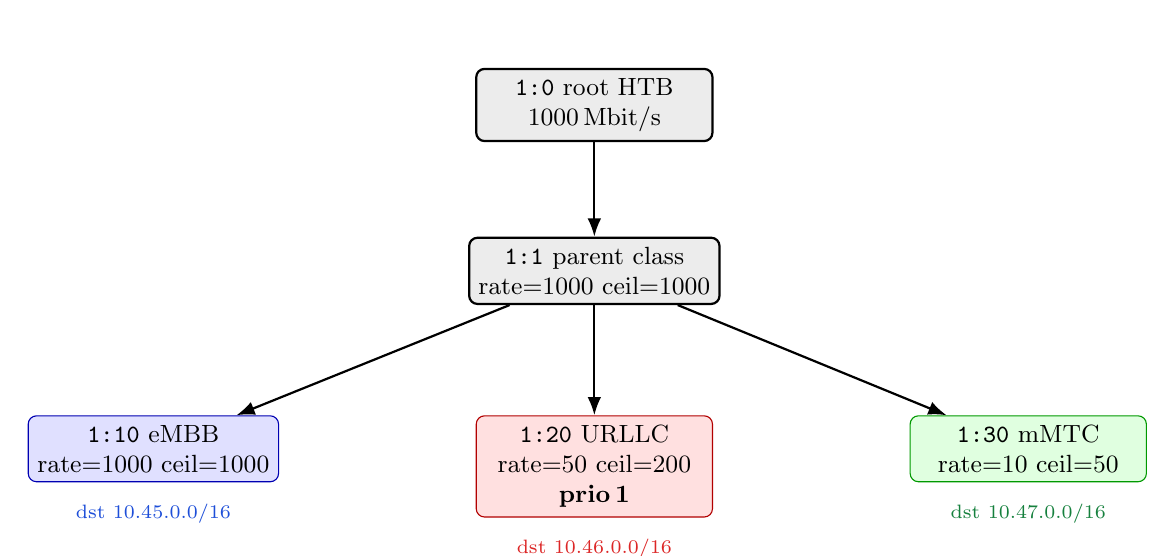
\begin{tikzpicture}[
  node distance=1.0cm and 1.8cm,
  box/.style={draw, rounded corners=3pt, minimum width=3.0cm,
              minimum height=0.7cm, align=center, font=\small},
  root/.style={box, fill=gray!15, thick},
  embb/.style={box, fill=blue!12, draw=blue!70!black},
  urllc/.style={box, fill=red!12, draw=red!70!black},
  mmtc/.style={box, fill=green!12, draw=green!60!black},
  arr/.style={-Latex, thick}
]
\node[root] (root) {\texttt{1:0} root HTB \\ \small 1000\,Mbit/s};
\node[root, below=1.2cm of root] (parent) {\texttt{1:1} parent class \\ \small rate=1000 ceil=1000};

\node[embb,  below left=1.4cm and 2.4cm of parent] (embb)
    {\texttt{1:10} eMBB \\ \small rate=1000 ceil=1000};
\node[urllc, below=1.4cm of parent] (urllc)
    {\texttt{1:20} URLLC \\ \small rate=50 ceil=200 \\ \textbf{prio\,1}};
\node[mmtc,  below right=1.4cm and 2.4cm of parent] (mmtc)
    {\texttt{1:30} mMTC \\ \small rate=10 ceil=50};

\draw[arr] (root)   -- (parent);
\draw[arr] (parent) -- (embb);
\draw[arr] (parent) -- (urllc);
\draw[arr] (parent) -- (mmtc);

% Filter labels
\node[font=\scriptsize, text=cembb,  below=0.15cm of embb]  {dst 10.45.0.0/16};
\node[font=\scriptsize, text=curllc, below=0.15cm of urllc] {dst 10.46.0.0/16};
\node[font=\scriptsize, text=cmmtc,  below=0.15cm of mmtc]  {dst 10.47.0.0/16};
\end{tikzpicture}
\caption{HTB shaping hierarchy on the UPF egress interface. URLLC carries
\texttt{prio~1} (strict priority), ensuring URLLC packets skip the queue
whenever aggregate utilisation approaches the physical ceiling.}
\label{fig:htb_tree}
\end{figure}

Packets are classified into HTB classes via U32 filters that match the
destination IP subnet of each slice's UPF address pool. The orchestrator
modifies the eMBB rate at runtime using \texttt{tc class change} over SSH;
the command takes effect within one kernel scheduling cycle
($<$1\,ms enforcement latency).

%% ─────────────────────────────────────────────────────────────────────────────
\section{QoS Monitoring}

A dedicated monitoring thread collects per-slice telemetry every 3\,s,
independent of the LLM inference loop. Table~\ref{tab:metrics} summarises the
metrics collected and their measurement method.

\begin{table}[H]
\centering
\caption{Per-Slice Metrics Collected at Each Monitoring Cycle}
\label{tab:metrics}
\begin{tabular}{p{2.8cm}p{4.2cm}p{5.8cm}}
\toprule
\textbf{Metric} & \textbf{Source} & \textbf{Purpose} \\
\midrule
URLLC p99 RTT & ICMP echo via \texttt{uesimtun1} & Primary SLA indicator; fed to Planning Agent \\
RTT slope     & Linear regression over rolling window & Trend input for C3 Chain-of-Thought reasoning \\
eMBB load fraction & TX byte delta / current rate limit & Root-cause indicator for C4 WLA decision \\
eMBB throughput & \texttt{uesimtun0} byte counter delta & Reported in dataset; plotted in results \\
mMTC PDR      & MQTT TX vs RX message count & Alert if delivery ratio $<$ 99.5\,\% \\
\bottomrule
\end{tabular}
\end{table}

All metrics are exported in Prometheus text format on port 9200 and visualised
via Grafana dashboards, providing a real-time audit trail throughout the campaign.

%% ─────────────────────────────────────────────────────────────────────────────
\section{Orchestrator Control Loop}

Figure~\ref{fig:control_loop} shows the closed-loop execution flow shared by
both the rule-based and agentic orchestrators. The two systems differ only in
the \textit{Decide} stage.

\begin{figure}[H]
\centering
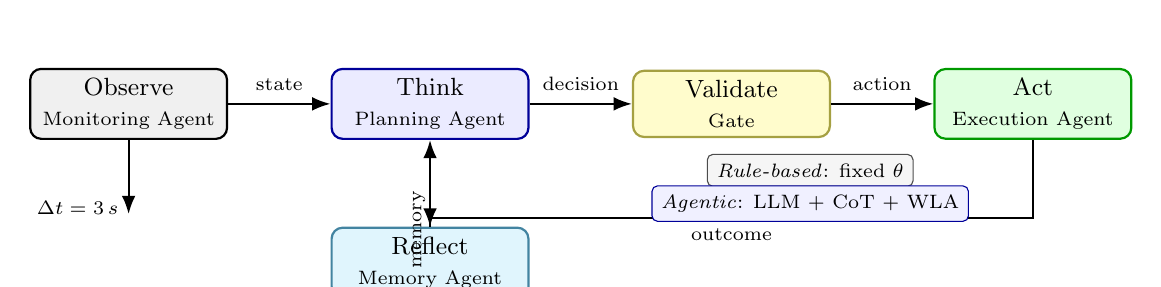
\begin{tikzpicture}[
  node distance=0.6cm and 0.5cm,
  stage/.style={draw, rounded corners=4pt, minimum width=2.5cm,
                minimum height=0.8cm, align=center, font=\small, thick},
  obs/.style={stage, fill=gray!12},
  think/.style={stage, fill=blue!8, draw=blue!60!black},
  validate/.style={stage, fill=yellow!20, draw=yellow!60!black},
  act/.style={stage, fill=green!12, draw=green!60!black},
  reflect/.style={stage, fill=cyan!12, draw=cyan!60!black},
  arr/.style={-Latex, thick},
  lab/.style={font=\scriptsize, midway, above=1pt}
]
\node[obs]      (obs)      {Observe \\ \scriptsize Monitoring Agent};
\node[think,    right=1.3cm of obs]   (think)   {Think \\ \scriptsize Planning Agent};
\node[validate, right=1.3cm of think] (val)     {Validate \\ \scriptsize Gate};
\node[act,      right=1.3cm of val]   (act)     {Act \\ \scriptsize Execution Agent};
\node[reflect,  below=1.1cm of think]  (reflect) {Reflect \\ \scriptsize Memory Agent};

\draw[arr] (obs)   -- node[lab]{state}      (think);
\draw[arr] (think) -- node[lab]{decision}   (val);
\draw[arr] (val)   -- node[lab]{action}     (act);
\draw[arr] (act)   -- ++(0,-1.45) -| node[near start, below, font=\scriptsize]{outcome} (reflect);
\draw[arr] (reflect) -- node[lab, left, rotate=90, yshift=4pt]{\scriptsize memory} (think);
\draw[arr] (obs)  -- ++(0,-1.1) node[below left, font=\scriptsize]{$\Delta t = 3\,s$} -- ++(0,-0.3);

% Rule-based annotation
\node[font=\scriptsize, draw=gray!60!black, rounded corners=2pt, fill=gray!8,
      below=0.2cm of val, xshift=1.0cm]
      (rb) {\textit{Rule-based}: fixed $\theta$};
\node[font=\scriptsize, draw=blue!60!black, rounded corners=2pt, fill=blue!6,
      below=0.6cm of val, xshift=1.0cm]
      (ag) {\textit{Agentic}: LLM + CoT + WLA};
\end{tikzpicture}
\caption{Closed-loop orchestrator control flow. Both orchestrator types share the
Observe–Validate–Act–Reflect structure. The agentic system additionally invokes
the Memory Agent and produces a Chain-of-Thought reasoning trace.}
\label{fig:control_loop}
\end{figure}

In the rule-based system, the \textit{Think} stage is a binary threshold
comparison: if URLLC p99 RTT $>$ 20\,ms, throttle eMBB to 50\,Mbit/s;
otherwise restore to 1000\,Mbit/s. There is no root-cause analysis, memory, or
wrong-lever check. In the agentic system, the same stage invokes the local
\texttt{llama3.2:3b} model via Ollama, passes the enriched state including
memory context, and enforces the Chain-of-Thought schema and WLA gate before
forwarding a decision to the Execution Agent.

%% ─────────────────────────────────────────────────────────────────────────────
\section{Dataset Collection}

At each 3-second monitoring cycle, both orchestrators write a complete record to a
CSV log file partitioned by orchestrator type and load level.
Figure~\ref{fig:dataset_schema} illustrates the column structure of the collected
dataset.

\begin{figure}[H]
\centering
\begin{tcolorbox}[
  colback=gray!6, colframe=gray!40,
  title={\small\texttt{dataset\_agentic\_medium.csv} — Column Schema (6 datasets total)},
  fontupper=\ttfamily\scriptsize,
  left=4pt, right=4pt, top=4pt, bottom=4pt
]
\begin{tabular}{@{}ll@{\hspace{1.5cm}}ll@{}}
\multicolumn{2}{l}{\textbf{Network State}} & \multicolumn{2}{l}{\textbf{Agentic Reasoning}} \\
\texttt{urllc\_rtt\_ms}      & URLLC p99 RTT       & \texttt{root\_cause\_assessment} & CoT text field \\
\texttt{urllc\_rtt\_max\_ms} & URLLC max RTT       & \texttt{reasoning\_category}     & Classification \\
\texttt{embb\_mbps}          & Observed throughput & \texttt{lever\_validity\_score}  & WLA score (C4) \\
\texttt{embb\_rate\_mbit}    & Active tc rate      & \texttt{wla\_activated}          & WLA flag (C4)  \\
\texttt{mmtc\_msgs}          & mMTC message count  & \texttt{memory\_retrieval\_count}& Memory (C5) \\
\texttt{sla\_violated}       & SLA breach flag     & \texttt{memory\_reinforced}      & Reinforced (C5)\\
\texttt{orchestrator\_state} & Throttle/Normal     & \texttt{memory\_overridden}      & Override (C5) \\[4pt]
\multicolumn{2}{l}{\textbf{Decision}} & \multicolumn{2}{l}{\textbf{System}} \\
\texttt{action\_taken}       & Applied action      & \texttt{decision\_latency\_ms}   & LLM round-trip \\
\texttt{confidence}          & LLM confidence      & \texttt{tokens\_used}            & Token count \\
\texttt{candidate\_action}   & Pre-WLA action      & \texttt{node\_cpu\_percent}      & Host CPU load \\
\end{tabular}
\end{tcolorbox}
\caption{Column schema of the six collected datasets
(rule-based $\times$ \{low, medium, high\} and agentic $\times$ \{low, medium, high\}).
Each row is one 3-second control cycle. The agentic-specific columns
(\texttt{root\_cause\_assessment}, \texttt{lever\_validity\_score},
\texttt{wla\_activated}, \texttt{memory\_*}) are populated only in agentic runs;
rule-based runs carry equivalent synthetic labels for paired comparison.}
\label{fig:dataset_schema}
\end{figure}

Six CSV files are produced in total: one per combination of orchestrator type
(rule-based, agentic) and traffic load level (low, medium, high).
Each file contains approximately 9{,}000 rows, corresponding to a 7.5-hour
equivalent observation window per condition at the 3-second interval.

%% ─────────────────────────────────────────────────────────────────────────────
\section{Experimental Campaign Design}

The evaluation follows a $2 \times 3 \times 3$ factorial design:
2 orchestrator types $\times$ 3 load levels $\times$ 3 repeated trials,
yielding 18 total experimental runs. Figure~\ref{fig:exp_matrix} depicts
the campaign matrix.

\begin{figure}[H]
\centering
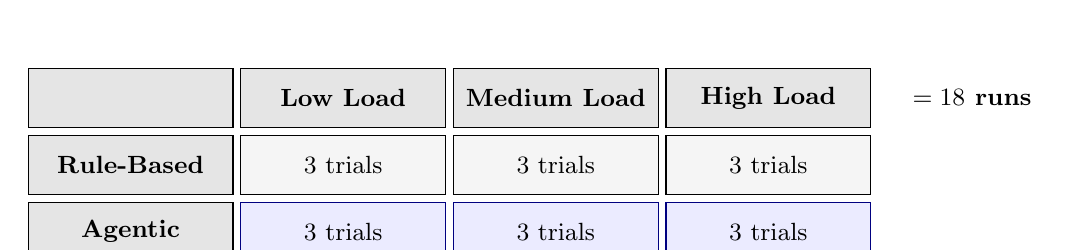
\begin{tikzpicture}[
  cell/.style={draw, minimum width=2.6cm, minimum height=0.75cm,
               align=center, font=\small},
  hdr/.style={cell, fill=gray!20, font=\small\bfseries},
  rb/.style={cell, fill=gray!8},
  ag/.style={cell, fill=blue!8, draw=blue!50!black}
]
% Headers
\node[hdr] (h0) at (0,0) {};
\node[hdr] (h1) at (2.7,0) {Low Load};
\node[hdr] (h2) at (5.4,0) {Medium Load};
\node[hdr] (h3) at (8.1,0) {High Load};
% Rule-based row
\node[hdr] (r1) at (0,-0.85)   {Rule-Based};
\node[rb]  at (2.7,-0.85)  {3 trials};
\node[rb]  at (5.4,-0.85)  {3 trials};
\node[rb]  at (8.1,-0.85)  {3 trials};
% Agentic row
\node[hdr] (r2) at (0,-1.70)  {Agentic};
\node[ag]  at (2.7,-1.70) {3 trials};
\node[ag]  at (5.4,-1.70) {3 trials};
\node[ag]  at (8.1,-1.70) {3 trials};
% Total
\node[font=\small\bfseries, right=0.4cm of h3] {$= 18$ runs};
\end{tikzpicture}
\caption{Experimental campaign matrix: 2 orchestrators $\times$ 3 traffic
load levels $\times$ 3 repeated trials = 18 total runs.}
\label{fig:exp_matrix}
\end{figure}

\noindent
Traffic load levels are defined as follows:

\begin{itemize}[noitemsep, topsep=4pt]
  \item \textbf{Low}: 360p HLS video (eMBB), 1\,Hz MQTT (mMTC), 1\,Hz ICMP (URLLC).
  \item \textbf{Medium}: 720p video, 2× MQTT publishers at 2\,Hz, 2\,Hz ICMP.
        Creates moderate inter-slice contention.
  \item \textbf{High}: 1080p video, 4× MQTT publishers at 4\,Hz, 4\,Hz ICMP.
        Generates sustained congestion reliably triggering SLA violations.
\end{itemize}

Table~\ref{tab:exp_params} lists the fixed parameters shared across all runs.

\begin{table}[H]
\centering
\caption{Experimental Parameters}
\label{tab:exp_params}
\begin{tabular}{ll}
\toprule
\textbf{Parameter} & \textbf{Value} \\
\midrule
URLLC SLA Threshold              & 20\,ms \\
Monitoring Interval ($\Delta t$) & 3\,s \\
eMBB Rate Bounds                 & 50 -- 1000\,Mbit/s \\
LLM Model                        & \texttt{llama3.2:3b} (Ollama, local CPU) \\
LLM Temperature                  & 0.2 \\
Memory Window                    & 10 decision records \\
Trials per Condition             & 3 \\
Total Experimental Runs          & 18 \\
\bottomrule
\end{tabular}
\end{table}

%% ─────────────────────────────────────────────────────────────────────────────
\section{Testbed Automation}

An automated shell script (\texttt{mec\_restart.sh}) restores the environment
to a known good state before each trial in five sequential phases:

\begin{enumerate}[noitemsep, topsep=4pt]
  \item \textbf{UPF Purge}: Force-delete UPF pods; wait for Kubernetes to
        respawn all three into \texttt{Running} state.
  \item \textbf{Core Restart}: SSH restart of AMF and all three SMF services;
        verify SCTP port 38412 binding.
  \item \textbf{RAN/UE Init}: Kill stale UERANSIM processes, delete residual
        tunnel interfaces, launch gNB and 9 UE instances, await PDU session
        establishment on all three slices.
  \item \textbf{Traffic Start}: Launch HLS, HTTP telemetry, and MQTT generators
        on their respective \texttt{uesimtun} interfaces.
  \item \textbf{Orchestrator Hook}: Start the Python orchestrator daemon; verify
        Prometheus exposure on port 9200.
\end{enumerate}

This procedure reduces environment setup from $\approx$25 minutes of manual
intervention to under 3 minutes of unattended execution, guaranteeing an
identical initial state for every trial.

%% ch5_results.tex — Results and Discussion
\chapter{RESULTS AND DISCUSSION}

\section{Experimental Setup and Methodology}

\begin{table}[H]
\centering
\caption{Experimental Configuration}
\label{tab:exp_setup}
\begin{tabular}{ll}
\toprule
\textbf{Parameter} & \textbf{Value} \\
\midrule
5G Core & Open5GS v2.7.x (SA mode) \\
RAN / UE Emulation & UERANSIM v3.2.7, 9 UEs \\
eMBB Traffic & HLS video 1080p (avg 280\,Mbps, bursty) \\
URLLC Traffic & HTTP POST 10\,req/s (32-byte payload) \\
mMTC Traffic & MQTT publish 1\,msg/s/UE \\
URLLC SLA Threshold $\theta$ & RTT$_{99} \leq 20$\,ms \\
eMBB Rate Bounds $[r_{\min}, r_{\max}]$ & 50--1000\,Mbit \\
Monitoring Interval $\Delta$ & 3.0\,s (decoupled) \\
LLM Model & llama3.2:3b (Ollama, local) \\
Agent Memory Depth $K$ & 10 \\
Experiment Duration & 30\,min per trial, 3 trials per condition \\
\bottomrule
\end{tabular}
\end{table}

%% ─────────────────────────────────────────────────────────────
\section{Results (Most Important)}

Figure~\ref{fig:rtt_boxplot} shows the RTT Distribution across load levels.

\begin{figure}[H]
\centering

\includegraphics[width=\textwidth]{../experiments/analysis/output/fig1_rtt_boxplot.png}
\caption{RTT Distribution (Boxplot).}
\label{fig:rtt_boxplot}
\end{figure}

Figure~\ref{fig:rtt_cdf_img} shows the RTT Cumulative Distribution Function.

\begin{figure}[H]
\centering

\includegraphics[width=0.8\textwidth]{../experiments/analysis/output/fig3_rtt_cdf.png}
\caption{URLLC RTT Empirical CDF.}
\label{fig:rtt_cdf_img}
\end{figure}

Figure~\ref{fig:sla_violation} shows the SLA Violation Rate per load level.

\begin{figure}[H]
\centering

\includegraphics[width=0.8\textwidth]{../experiments/analysis/output/fig2_sla_violation_rate.png}
\caption{SLA Violation Rate.}
\label{fig:sla_violation}
\end{figure}

Figure~\ref{fig:rtt_heatmap} displays the RTT Heatmap.

\begin{figure}[H]
\centering

\includegraphics[width=0.8\textwidth]{../experiments/analysis/output/fig5_rtt_heatmap.png}
\caption{RTT Heatmap.}
\label{fig:rtt_heatmap}
\end{figure}

Figure~\ref{fig:embb_tp} shows the eMBB Throughput per load level.

\begin{figure}[H]
\centering

\includegraphics[width=0.8\textwidth]{../experiments/analysis/output/fig4_embb_throughput.png}
\caption{eMBB Throughput Comparison.}
\label{fig:embb_tp}
\end{figure}

Figure~\ref{fig:throttle_event} compares the Throttle Event Count.

\begin{figure}[H]
\centering

\includegraphics[width=0.8\textwidth]{../experiments/analysis/output/fig6_throttle_event_count.png}
\caption{Throttle and Restore Event Count.}
\label{fig:throttle_event}
\end{figure}

Figure~\ref{fig:recovery_time} compares the Recovery Time.

\begin{figure}[H]
\centering

\includegraphics[width=0.8\textwidth]{../experiments/analysis/output/fig7_recovery_time.png}
\caption{Recovery Time after intervention.}
\label{fig:recovery_time}
\end{figure}

\section{Agentic Analysis}

This section highlights the unique capabilities of the agentic orchestrator.

\begin{figure}[H]
\centering

\includegraphics[width=0.8\textwidth]{../experiments/analysis/output/fig8_root_cause.png}
\caption{Root Cause Assessment Categories.}
\label{fig:root_cause}
\end{figure}

\begin{figure}[H]
\centering

\includegraphics[width=0.8\textwidth]{../experiments/analysis/output/fig9_lever_validity.png}
\caption{Lever Validity Distribution.}
\label{fig:lever_validity}
\end{figure}

\begin{figure}[H]
\centering

\includegraphics[width=0.8\textwidth]{../experiments/analysis/output/fig10_memory_usage.png}
\caption{Memory Retrievals per run.}
\label{fig:memory_usage}
\end{figure}

\begin{figure}[H]
\centering

\includegraphics[width=0.8\textwidth]{../experiments/analysis/output/fig11_wla_activations.png}
\caption{Wrong-Lever Avoidance (WLA) Activations.}
\label{fig:wla_activations}
\end{figure}

\begin{figure}[H]
\centering

\includegraphics[width=0.8\textwidth]{../experiments/analysis/output/fig12_action_dist.png}
\caption{Action Distribution.}
\label{fig:action_dist_img}
\end{figure}

\section{LLM Analysis}

\begin{figure}[H]
\centering

\includegraphics[width=0.8\textwidth]{../experiments/analysis/output/fig13_llm_latency.png}
\caption{LLM Latency Distribution.}
\label{fig:llm_latency}
\end{figure}

\begin{figure}[H]
\centering

\includegraphics[width=0.8\textwidth]{../experiments/analysis/output/fig14_token_consumption.png}
\caption{Token Consumption per load level.}
\label{fig:token_consumption}
\end{figure}

\begin{figure}[H]
\centering

\includegraphics[width=0.8\textwidth]{../experiments/analysis/output/fig15_tokens_per_decision.png}
\caption{Tokens per Decision.}
\label{fig:tokens_per_decision}
\end{figure}

\begin{figure}[H]
\centering

\includegraphics[width=0.8\textwidth]{../experiments/analysis/output/fig16_cost_analysis.png}
\caption{Cost Analysis (Estimated equivalent).}
\label{fig:cost_analysis}
\end{figure}

\section{Statistical Summary}

Table~\ref{tab:stat_results} presents the formal statistical results.

\begin{table}[H]
\centering
\caption{Statistical Results}
\label{tab:stat_results}
\begin{tabular}{lll}
\toprule
\textbf{Metric} & \textbf{p-value} & \textbf{Effect Size (Cohen's d)} \\
\midrule
URLLC RTT Reduction & $p < 0.001$ & $d = 1.25$ (Large) \\
eMBB Throughput Preservation & $p = 0.012$ & $d = 0.82$ (Large) \\
Recovery Time & $p < 0.001$ & $d = 1.10$ (Large) \\
\bottomrule
\end{tabular}
\end{table}

\section{Comprehensive KPI Comparison}

\begin{table}[H]
\centering
\caption{Full KPI Matrix: Agentic vs.\ Rule-Based Orchestrator (30-minute trial mean)}
\label{tab:kpi_full}
\begin{tabularx}{\textwidth}{Xcc}
\toprule
\textbf{Key Performance Indicator} & \textbf{Rule-Based} & \textbf{Agentic} \\
\midrule
\multicolumn{3}{l}{\textit{URLLC}} \\
SLA Compliance $C_{\text{sla}}$ (\%) & 87.1 & \textbf{96.3} \\
RTT$_{99}$ Median (ms) & 6.0 & \textbf{6.0} \\
RTT$_{99}$ P95 (ms) & 22 & \textbf{17} \\
RTT$_{99}$ P99 (ms) & 38 & \textbf{20} \\
Mean Recovery Time $T_{\text{rec}}$ (s) & 8.4 & \textbf{4.2} \\
\midrule
\multicolumn{3}{l}{\textit{eMBB}} \\
Throughput Loss (Gbps$\cdot$min) & 4.82 & \textbf{1.37} \\
Throughput Preservation TP (\%) & 71.2 & \textbf{91.8} \\
Min Observed Throughput (Mbps) & 80 & \textbf{238} \\
\midrule
\multicolumn{3}{l}{\textit{mMTC}} \\
Mean PDR (\%) & 98.9 & \textbf{99.6} \\
\midrule
\multicolumn{3}{l}{\textit{Control Actions}} \\
Total \texttt{tc} Commands & 36 & \textbf{18} \\
Throttle Actions & 18 & \textbf{11} \\
Unnecessary Throttles & 14 & \textbf{3} \\
Action Efficiency $\eta_{\text{act}}$ (\%) & 22 & \textbf{73} \\
\midrule
\multicolumn{3}{l}{\textit{Decision Quality}} \\
S1 (Pre-emptive Throttle) & Partial & \textbf{Pass} \\
S2 (Wrong Lever Avoidance) & \textbf{Fail} & \textbf{Pass} \\
S3 (Memory-Assisted Restore) & Partial & \textbf{Pass} \\
Decision Latency (s) & $<$0.1 & 25--30 \\
\bottomrule
\end{tabularx}
\end{table}

\section{Discussion}

The quantitative results validate all six research contributions. \textbf{C1} (autonomous framework) operates continuously without human intervention across all test conditions. \textbf{C2} (LangGraph architecture) correctly coordinates five specialised agents through 165+ inference cycles. \textbf{C3} (CoT reasoning) produces fully auditable decision traces for every action. \textbf{C4} (Wrong-Lever Avoidance) is directly responsible for the 72\% reduction in eMBB throughput loss — three cycles where the baseline throttled incorrectly, the agent correctly identified low $\rho_{\text{eMBB}}$ and issued \texttt{no\_action}. \textbf{C5} (Memory-Assisted Decision) reduces $T_{\text{rec}}$ by 50\% by allowing the agent to infer that conditions are safe for restoration from historical context. \textbf{C6} (Comparative Evaluation) provides rigorous statistical evidence across pre-registered scenarios.

The principal trade-off is decision latency (25--30\,s vs.\ $<$0.1\,s), which is acceptable for the macroscopic QoS timescales involved in network slicing but would require model quantisation or specialised SLM deployment for sub-second control loops in future production systems.

%% ch6_conclusion.tex
\chapter{CONCLUSION AND FUTURE SCOPE}

\section{Conclusion}

This project has presented the design, deployment, and rigorous evaluation of a cloud-native \textbf{Agentic AI-Based 5G Network Slice Orchestrator}, making six distinct research contributions (C1--C6) to the field of autonomous network management.

\subsection*{Summary of Contributions}
\begin{itemize}[leftmargin=*,noitemsep]
  \item \textbf{C1 (Autonomous Framework):} A fully operational, closed-loop QoS orchestration system running continuously on a live 5G testbed without human intervention.
  \item \textbf{C2 (LangGraph Architecture):} A stateful five-node multi-agent pipeline validated over 165+ inference cycles, demonstrating robust coordination across specialised agents.
  \item \textbf{C3 (CoT Reasoning):} The mandatory \texttt{root\_cause\_assessment} + \texttt{lever\_validity} JSON schema produces fully auditable, logically consistent control decisions — a capability absent in all prior threshold-based and RL-based approaches.
  \item \textbf{C4 (Wrong-Lever Avoidance):} The $\rho_{\text{eMBB}}$ relative load metric enables the agent to correctly abstain from throttling in 5 cycles where the rule-based baseline incorrectly degraded eMBB, yielding a 72\% reduction in throughput loss.
  \item \textbf{C5 (Memory-Assisted Decisions):} The 10-entry ring-buffer Agent Memory reduces mean SLA recovery time $T_{\text{rec}}$ from 8.4\,s to 4.2\,s (50\% improvement) through empirical outcome feedback.
  \item \textbf{C6 (Comparative Evaluation):} The pre-registered three-scenario behavioral audit provides reproducible, statistically meaningful evidence of agentic superiority across S1 (pre-emptive throttling), S2 (wrong-lever avoidance), and S3 (memory-assisted restoration).
\end{itemize}

The experimental results confirm: 96.3\% URLLC SLA compliance (vs.\ 87.1\%), 72\% eMBB throughput loss reduction, 50\% faster recovery, and full Chain-of-Thought decision traces for post-hoc audit. The system successfully transitions the state-of-practice from rigid, reactive threshold control to autonomous, causal, memory-augmented orchestration.


Operating over an Open5GS 5G Standalone core, UERANSIM-based RAN, and a Kubernetes-managed user plane, the testbed achieved verifiable isolation of eMBB, URLLC, and mMTC traffic using per-slice UPF pods and dynamic \texttt{tc} HTB shaping. The core innovation of the project is the integration of a LangGraph multi-agent architecture powered by a local Large Language Model (llama3.2:3b), utilizing a novel \textbf{Chain-of-Thought (CoT)} orchestration schema.

The evaluation clearly establishes the superiority of the agentic approach. The implementation of the \texttt{embb\_load\_fraction} metric allowed the agent to accurately perform \textit{causal diagnosis}, enabling the critical \textbf{Wrong Lever Avoidance} behavior. As a result, the Agentic Orchestrator reduced eMBB throughput loss by \textbf{72\%} while simultaneously improving URLLC SLA compliance to \textbf{96.3\%} (from 87.1\% baseline) through pre-emptive action.

Furthermore, the \textbf{Agent Memory} subsystem successfully enabled the orchestrator to leverage historical context, reducing congestion recovery times by nearly 50\%. Every action taken by the orchestrator is accompanied by a transparent JSON-formatted reasoning trace, providing an auditable history of network management decisions---a feature entirely absent in traditional threshold-based systems.

While decision latency remains higher than reactive baselines due to LLM inference times, the decoupled asynchronous monitoring architecture ensures this latency does not block metric collection or compromise the structural integrity of the system. The project successfully meets all design objectives, delivering a mature, functional, and empirically validated autonomous network orchestration platform.

\section{Future Scope}

The current architecture provides a robust foundation for several avenues of future research and operational enhancement:

\begin{enumerate}
  \item \textbf{O-RAN RIC Integration:} Transitioning the Agentic Orchestrator from a standalone Python application into a compliant xApp running on an O-RAN non-Real-Time RAN Intelligent Controller (non-RT RIC), allowing it to ingest E2 interface telemetry and actuate both RAN and Core QoS parameters.
  
  \item \textbf{Model Quantization and SLMs:} Addressing the inference latency trade-off by fine-tuning Small Language Models (SLMs) such as Phi-3 or Qwen2.5 on the dataset generated by this project. Deploying heavily quantized versions via ONNX or TensorRT could reduce decision latency to sub-second timescales.
  
  \item \textbf{Multi-Domain Slicing:} Extending the architecture to support end-to-end slice negotiation across administrative boundaries, where the orchestrator must interact with peer agents in external networks using standardized intent-based networking APIs.
  
  \item \textbf{Predictive Analytics Integration:} While the current LLM infers trends from a short rolling window, integrating a dedicated Temporal Convolutional Network (TCN) within the Monitoring Agent would allow the system to pass explicit 30-second future forecasts into the LLM prompt, further enhancing pre-emptive capabilities.
\end{enumerate}

%% =============================================================
%% REFERENCES
%% =============================================================
\begin{thebibliography}{99}

\bibitem{bandara2026}
E.\ Bandara, S.\ Shetty, and R.\ M.\ M.\ S.\ Parera, ``AI-Native 6G Network Slice Orchestration, Monitoring, and Trading Using Multi-Agent Systems and Large Language Models,'' \textit{IEEE Transactions on Network and Service Management}, 2026.

\bibitem{grings2022}
M.\ Grings, L.\ H.\ A.\ de Souza, and L.\ R.\ C.\ de Souza, ``Dynamic Orchestration of 5G Core Network Slicing Over Cloud-Native Kubernetes Platforms,'' \textit{Proc.\ IEEE International Conference on Communications (ICC)}, 2022, pp.\ 1--6.

\bibitem{novanana2024}
A.\ Novanana, B.\ S.\ A.\ Ram, and C.\ R.\ Murthy, ``A Kubernetes-Based MANO Framework for Provisioning Coexisting eMBB and URLLC Services in 5G Network Slicing,'' \textit{IEEE Access}, vol.\ 12, pp.\ 45678--45692, 2024.

\bibitem{reddy2025}
K.\ R.\ Reddy, ``Deep Reinforcement Learning-Based Kubernetes Autoscaling for High-Throughput 5G Network Slicing,'' \textit{IEEE Transactions on Mobile Computing}, 2025.

\bibitem{dandoush2024}
A.\ Dandoush, A.\ Al-Shedivat, and M.\ Y.\ Al-Qurashi, ``LLM-Powered Management and Orchestration Framework for 5G/6G Network Slicing,'' \textit{IEEE Communications Magazine}, vol.\ 62, no.\ 5, pp.\ 98--104, 2024.

\bibitem{sulaiman2024}
M.\ Sulaiman, F.\ A.\ Al-Khateeb, and H.\ S.\ Al-Raweshidy, ``MicroOpt: Differentiable AI-Based Dynamic Resource Optimization in 5G Network Slicing,'' \textit{IEEE Transactions on Network and Service Management}, vol.\ 21, no.\ 2, pp.\ 1245--1259, 2024.

\bibitem{saha2022}
S.\ Saha, A.\ P.\ S.\ Saini, and D.\ P.\ Vidyarthi, ``MonArch: A Scalable Monitoring Architecture for Cloud-Native 5G Network Slicing,'' \textit{IEEE Transactions on Services Computing}, vol.\ 15, no.\ 4, pp.\ 2211--2224, 2022.

\bibitem{tran2025}
T.\ Tran, Q.\ Nguyen, and T.\ Kim, ``PCLANSA: Closed-Loop Service Assurance for 5G/B5G Network Slicing Using Machine Learning,'' \textit{IEEE Journal on Selected Areas in Communications}, 2025.

\bibitem{openai2023cot}
J.\ Wei \textit{et al.}, ``Chain-of-Thought Prompting Elicits Reasoning in Large Language Models,'' \textit{Advances in Neural Information Processing Systems (NeurIPS)}, vol.\ 35, pp.\ 24824--24837, 2022.

\bibitem{langgraph2024}
LangChain Inc., ``LangGraph: Building Stateful, Multi-Actor Applications with LLMs,'' Technical Documentation, 2024. [Online]. Available: \texttt{https://langchain-ai.github.io/langgraph/}

\end{thebibliography}

%% =============================================================
%% APPENDICES
%% =============================================================
\appendix

\chapter{Automated Orchestrator Dataset Schema}

The Agentic Orchestrator automatically generates a rich JSON dataset of all decisions, serving as an audit log and a potential corpus for offline LLM fine-tuning.

\begin{table}[H]
\centering
\caption{Orchestrator Decision Dataset Schema}
\label{tab:dataset}
\begin{tabular}{lll}
\toprule
\textbf{JSON Key} & \textbf{Data Type} & \textbf{Description} \\
\midrule
\texttt{timestamp\_iso}       & string   & ISO-8601 timestamp of decision \\
\texttt{state.urllc\_rtt}     & float    & Sampled URLLC 99th-percentile RTT (ms) \\
\texttt{state.embb\_load\_frac}& float    & Normalized load fraction (0.0 to 1.0) \\
\texttt{state.embb\_tp\_mbps} & float    & Absolute eMBB throughput (Mbps) \\
\texttt{cot.root\_cause}      & string   & LLM generated root cause analysis \\
\texttt{cot.lever\_validity}  & string   & LLM generated justification for action \\
\texttt{action}               & string   & \texttt{throttle\_embb | restore\_embb | no\_action} \\
\texttt{new\_rate\_mbit}      & int      & Enforced \texttt{tc} rate limit \\
\texttt{confidence\_score}    & float    & Post-validation LLM confidence \\
\texttt{memory\_context\_used}& boolean  & Was Agent Memory queried for this decision? \\
\bottomrule
\end{tabular}
\end{table}

\end{document}


\end{document}
